
%%%%%%%%%%%%%%%%%%%%%%% file typeinst.tex %%%%%%%%%%%%%%%%%%%%%%%%%
%
% This is the LaTeX source for the instructions to authors using
% the LaTeX document class 'llncs.cls' for contributions to
% the Lecture Notes in Computer Sciences series.
% http://www.springer.com/lncs       Springer Heidelberg 2006/05/04
%
% It may be used as a template for your own input - copy it
% to a new file with a new name and use it as the basis
% for your article.
%
% NB: the document class 'llncs' has its own and detailed documentation, see
% ftp://ftp.springer.de/data/pubftp/pub/tex/latex/llncs/latex2e/llncsdoc.pdf
%
%%%%%%%%%%%%%%%%%%%%%%%%%%%%%%%%%%%%%%%%%%%%%%%%%%%%%%%%%%%%%%%%%%%


\documentclass[runningheads,a4paper]{llncs}


\setcounter{tocdepth}{4}

%\urldef{\mailsa}\path|{shengbo.guo}@xrce.xerox.com|
%\urldef{\mailsb}\path|{scott.sanner, wray.buntine}@nicta.com.au|
%\urldef{\mailsc}\path|{thore.graepel}@microsoft.com|
\newcommand{\keywords}[1]{\par\addvspace\baselineskip
\noindent\keywordname\enspace\ignorespaces#1}

%%%%%%%%%%%%%%%%%%%%% starting addition by Shengbo
%\usepackage{aistats2012}
%\usepackage[accepted]{aistats2e}
\usepackage{graphicx}
\usepackage{graphics}
\usepackage{amssymb}
\usepackage{amsmath}
%\usepackage{amsthm}
\usepackage{amsfonts}
\usepackage{amssymb}
\usepackage{subfigure}
\usepackage{epsfig}
\usepackage[hyphens]{url}
%\usepackage{hyperref}

\urldef{\mailsa}\path|{shengbo.guo}@xrce.xerox.com|
\urldef{\mailsb}\path|{scott.sanner, wray.buntine}@nicta.com.au|
\urldef{\mailsc}\path|{thore.graepel}@microsoft.com|
\newcommand{\unindent}{\hspace{-1mm}}
\newcommand{\unindentmore}{\hspace{-1.5mm}}
\def\argmax{\operatornamewithlimits{arg\,max}}
\def\argmin{\operatornamewithlimits{arg\,min}}
\long\def\COMMENT#1\ENDCOMMENT{\message{(Commented text...)}\par}

%\newtheorem{lemma}{Lemma}%[section]

%%%%%%%%%%%%%%%%%%%%% ending addition by Shengbo

\begin{document}

\mainmatter  % start of an individual contribution

% first the title is needed
\title{Score-based Bayesian Skill Learning}

% a short form should be given in case it is too long for the running head
\titlerunning{Score-based Bayesian Skill Learning}

% the name(s) of the author(s) follow(s) next
%
% NB: Chinese authors should write their first names(s) in front of
% their surnames. This ensures that the names appear correctly in
% the running heads and the author index.
%
\author{Shengbo Guo\inst{1} \and Scott Sanner\inst{2} \and Thore Graepel\inst{3} \and Wray Buntine\inst{2}}
%\author{Unknown authors}
%
\authorrunning{S. Guo, S. Sanner, T. Graepel, W. Buntine}
%\authorrunning{Unknown authors}
% (feature abused for this document to repeat the title also on left hand pages)

% the affiliations are given next; don't give your e-mail address
% unless you accept that it will be published
\institute{Xerox Research Centre Europe
\and NICTA and the Australian National University
\and Microsoft Research Cambridge}
%\institute{Unknown institute}
%
% NB: a more complex sample for affiliations and the mapping to the
% corresponding authors can be found in the file "llncs.dem"
% (search for the string "\mainmatter" where a contribution starts).
% "llncs.dem" accompanies the document class "llncs.cls".
%

\toctitle{Score-based Bayesian Skill Learning}
\tocauthor{S. Guo, S. Sanner, T. Graepel, W. Buntine}

\maketitle


\begin{abstract}
We extend the Bayesian skill rating system of TrueSkill to accommodate
score-based match outcomes. TrueSkill has proven to be a very
effective algorithm for matchmaking --- the process of pairing
competitors based on similar skill-level --- in competitive online
gaming.  However, for the case of two teams/players, TrueSkill only
learns from win, lose, or draw outcomes and cannot use additional
match outcome information such as scores.  To address this deficiency,
we propose novel Bayesian graphical models as extensions of TrueSkill
that (1) model player's offence and defence skills separately and (2)
model how these offence and defence skills interact to generate
score-based match outcomes.  We derive efficient (approximate)
Bayesian inference methods for inferring latent skills in these new
models and evaluate them on three real data sets including Halo 2 XBox
Live matches. Empirical evaluations demonstrate that the new
score-based models (a) provide more accurate win/loss probability
estimates than TrueSkill when training data is limited,
(b) provide competitive and often better win/loss classification
performance than TrueSkill, and (c) provide reasonable score outcome predictions with an
appropriate choice of likelihood --- prediction for which TrueSkill was not
designed, but which can be useful in many applications.
\keywords{variational inference, matchmaking, graphical models}
\end{abstract}

\section{Introduction}

In online gaming, it is important to pair players or teams of players
so as to optimise their gaming experience.  Game players often expect
competitors with comparable skills for the most enjoyable experience;
match experience can be compromised if one side consistently
outperforms the other.  \emph{Matchmaking} attempts to pair players
such that match results are close to being even or a draw.  Hence, a
prerequisite for good matchmaking is the ability to predict future
match results correctly from historical match outcomes --- a task
that is often cast in terms of latent skill learning.
%How to do
%this for matches with score-based outcomes is the question we address
%in this paper.

TrueSkill~\cite{herbrich06569} is a state-of-the-art Bayesian skill
learning system: it has been deployed in the Microsoft Xbox 360 online
gaming system for both matchmaking and player ranking.  For the case
of two teams/players, TrueSkill, like
Elo~\cite{elo78TheRatingOfChessPlayers}, is restricted to learn skills
from match outcomes in terms of win, lose, or draw (WLD).
While we conjecture that TrueSkill discards potentially
valuable skill information carried by score-based outcomes,
there are at least two arguments in favour of TrueSkill's WLD-based
skill learning approach:
\begin{itemize}
\item WLD-based systems can be applied to any game whose outcome space
is WLD, no matter what the underlying scoring system is.
\item In many games, the objective is not to win by the highest
score differential, but rather simply to win.  In this case,
it can be said that TrueSkill's skill modeling and learning from WLD
outcomes aligns well with the players' underlying objective.
\end{itemize}
%if the skill estimates of the system are revealed back to the
%players, there is a danger that the players may begin optimising their
%game play to influence their public skill estimate.  Hence, if the
%skill estimate is based on measurements other than the true game
%outcomes, this can lead to a distortion of the game's dynamics.
%However, if we assume that score information is available and
%estimated skill information is maintained privately, then it makes
%sense to attempt to exploit this additional score information in
On the other hand, we note that discarding score results
ignores two important sources of information:
\begin{itemize}
\item High (or low) score
differentials can provide insight into relative team strengths.
\item Two dimensional score outcomes (i.e., a score for each side) provide a
direct basis for inferring separate offense and defense strengths for
each team, hence permitting finer-grained modeling of performance against
future opponents.
%Peeking ahead, we note that the predictive
%improvements of score-based models over TrueSkill as shown in
%Section~\ref{sec:results} support this conjecture in many cases.
\end{itemize}

In this work, we augment the TrueSkill model of WLD skill learning to
learn from score-based outcomes.  We explore single skill models as
well as separate offense/defense skill models made possible via
score-based modeling.  We also investigate both Gaussian and Poisson
score likelihood models, deriving a novel variational update for
approximate Bayesian inference in the latter case.  We evaluate these
novel Bayesian score-based skill-learning models in comparison to
TrueSkill (for WLD outcomes) on three datasets: 14 years of match
outcomes for the UK Premier League, 11 years of match outcomes for the
Australian Football (Rugby) League (AFL), and three days covering
6,000+ online match outcomes in the Halo 2 XBox video game.  Empirical
evaluations demonstrate that the new score-based models (a) provide
more accurate win/loss probability estimates than TrueSkill (in terms
of information gain) with limited amounts of training data, (b)
provide competitive and often better win/loss classification
performance than TrueSkill (in terms of area under the curve), and (c)
provide reasonably accurate score predictions with an appropriate
likelihood --- prediction for which TrueSkill was not designed but
important in cases such as tournaments that rank (or break ties) by
points, professional sports betting and bookmaking, and game-play
strategy decisions that are dependent on final score projections.

\section{Skill Learning using TrueSkill}

Since our score-based Bayesian skill learning contributions build on
TrueSkill~\cite{herbrich06569}, we begin with a review of the
TrueSkill Bayesian skill-learning graphical model for two
single-player teams.  We note that TrueSkill itself allows for matches
involving more than two teams and learning team members' individual
performances, but these extensions are not needed for the application
domains considered in the paper.

Suppose there are $n$ teams available for pairwise matches in a
game.  Let $M=\{i,j\}$ specify the two teams participating in a match
and define the outcome $o \in \{ \textit{team-i-win},
\textit{team-j-win}, \textit{draw} \}$.  TrueSkill models the
probability $p(o|\vec{l},M)$ of $o$ given the skill
level vector $\vec{l} \in \mathbb{R}^n$
of the teams in $M$,
and estimates
posterior distributions of skill levels according to Bayes' rule
{\small \begin{align}
    p(\vec{l}|o,M) & \propto p(o|\vec{l},M) p(\vec{l}),
\label{eq:BayeTrueSkill}
\end{align}}
where a factorising Gaussian prior is assumed:
{\small \begin{align}
    p(\vec{l}) & :=\prod_{i=1}^{n}\mathcal{N}(l_i;\mu_i,\sigma_i^2).
\end{align}}
To model the likelihood $p(o|\vec{l},M)$,
each team $i$ is assumed to exhibit a stochastic performance variable $p_i \sim
\mathcal{N}(p_i;l_i,\beta^2)$ in the game~\footnote{\noindent Note that we sometimes abuse notations on the use of $p$, $p_i$ and $\vec{p}$. $p$ is a probability measure; $p_i$ and $\vec{p}$ represent performance variables. The meaning of them is clear from the context.}. From this we can model
the performance differential $d$ as an indicator function $p(d|\vec{p},M) = \delta(d = p_i - p_j)$
and finally the probability of each outcome $o$ given this
differential $d$:
{\small \begin{align}
p(o|d) & =
\begin{cases}
o = \textit{team-i-win}: & \mathbb{I}[d > \epsilon]\\
o = \textit{team-j-win}: & \mathbb{I}[d < -\epsilon]\\
o = \textit{draw}:       & \mathbb{I}[|d| \leq \epsilon],
\end{cases}
\end{align}}
where $\mathbb{I}[\cdot]$ is an indicator function. Then the likelihood $p(o|\vec{l},M)$ in~\eqref{eq:BayeTrueSkill}
can be written as
{\small \begin{align*} %\label{eq:trueskill_update}
p(o|\vec{l},M) = \int \cdots \int_{\mathbb{R}^n} \int_{-\infty}^{+\infty} p(o|d) p(d|\vec{p},M) \prod_{i=1}^n p(p_i|l_i) \, \mathrm{d}\vec{p} \, \mathrm{d}d.
\end{align*}}
The entire TrueSkill model relevant to $M$ is shown in the
factor graph of Figure~\ref{fig:trueskill} with $P(o|d)$ given
for the case of $o = \textit{team-i-win}$.
TrueSkill uses message passing %and expectation propagation (EP)
%\cite{minka01ExpectationUAI}
to infer the posterior distribution in~\eqref{eq:BayeTrueSkill} ---
note that the posterior over $l_i$ and $l_j$ will be
updated according to the match
outcome while the posterior over
$l_k$ ($k \notin \{ i,j \}$) will remain unchanged from
the prior.  An optimal message passing schedule in the TrueSkill
factor graph (Figure~\ref{fig:trueskill}) is provided in the caption;
the message along arrow 2 is a step function that leads to
intractability for exact inference and thus TrueSkill uses message
approximation via moment matching.

\begin{figure}[t!]
\vspace{-5mm}
\centerline{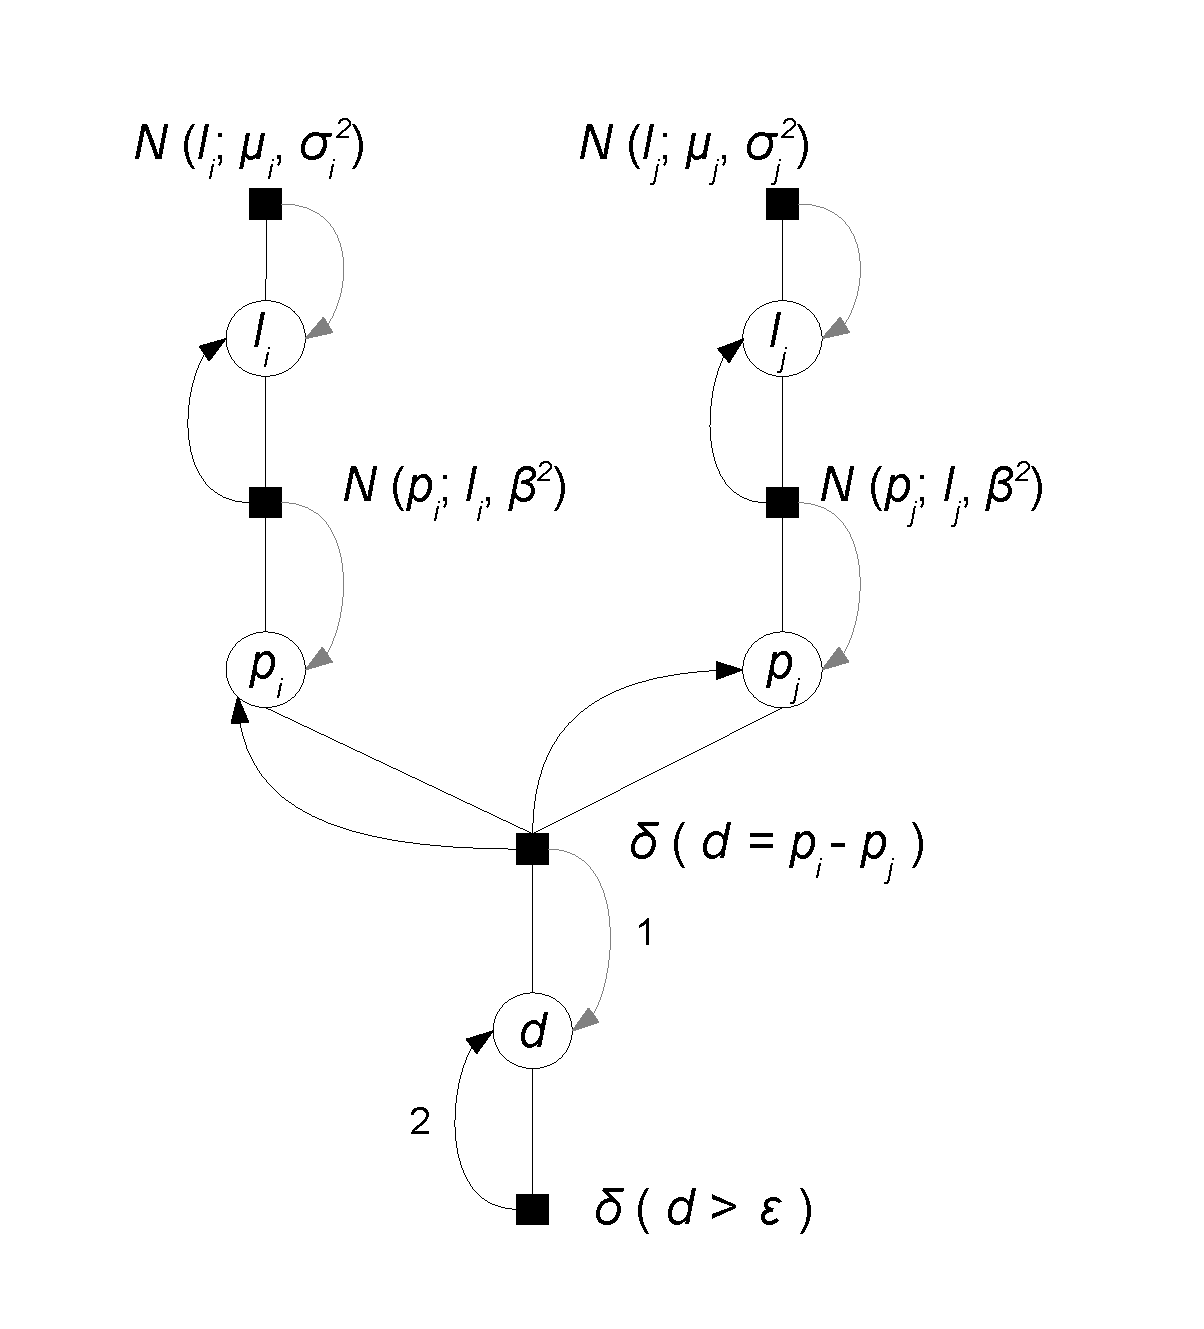
\includegraphics[scale=0.3]{TrueSkill}}
%\centerline{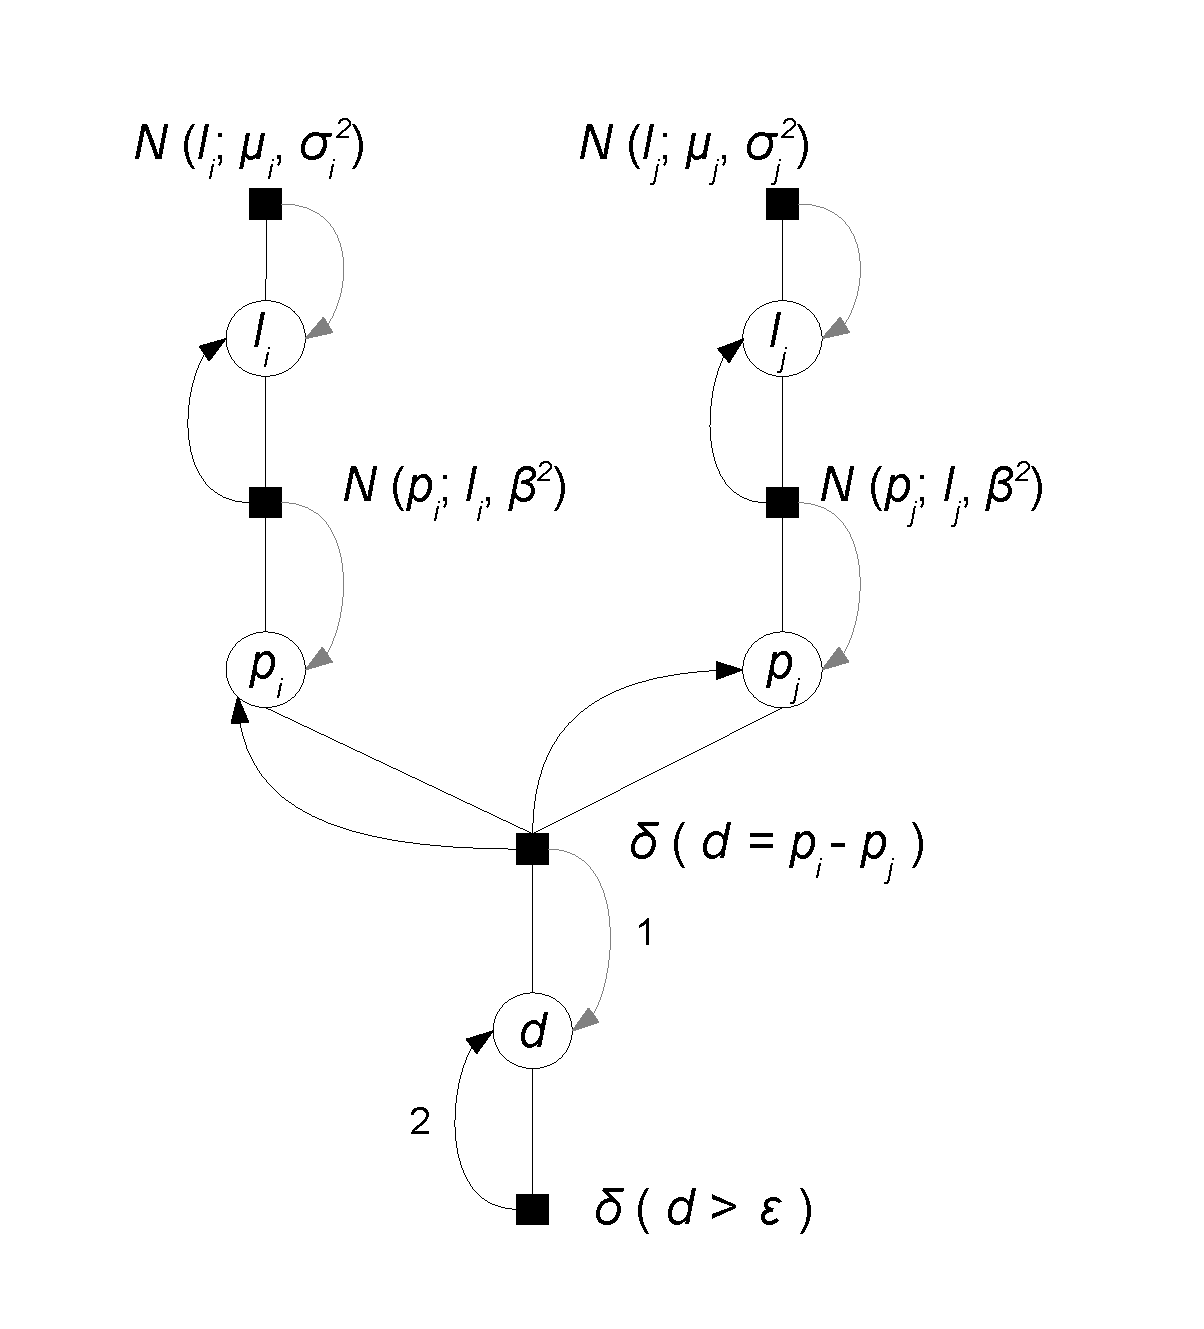
\includegraphics[scale=0.275]{TrueSkill}}
\vspace{-5mm}
\caption{\small TrueSkill factor graph for a match between two single-player
teams with team i winning.
There are three types of variables: $l_i$
for the skills of all players, $p_i$ for the performances of all
players and $d$ the performance difference. The first row of factors
encode the (product) prior; the product of the remaining factors
characterizes the likelihood for the game outcome team $i$ winning team $j$.
The arrows show the optimal message passing schedule: (1)
messages pass along \emph{gray} arrows from top to bottom, (2) the
marginal over $d$ is updated via message 1 followed by message 2
(which requires moment matching), (3) messages pass from bottom to top
along \emph{black} arrows.}
\label{fig:trueskill}
\vspace{-3mm}
\end{figure}

TrueSkill is an efficient and principled Bayesian skill learning
system.  However, due to its design goals, it discards score
information and does not take into account associated domain knowledge
such as offence/defence skill components.  Next,
we propose extensions of the TrueSkill factor graph and (approximate)
inference algorithms for score-based Bayesian skill learning, which
address these limitations.

\section{Score-based Bayesian Skill Models}
\label{sec:PoissonGaussianModels}

In this section, we introduce three graphical models as extensions for
the TrueSkill factor graph (Figure~\ref{fig:trueskill}) to incorporate
score-based outcomes in skill learning.  Our first two graphical
models are motivated by modeling score-based outcomes as generated by
separate offence and defence skills for each team.  The first
generative score model uses a Poisson, which is natural model when
scores are viewed as counts of scoring events.  The second generative
model uses a simpler Gaussian model.  Our third model is a simplified
version of the Gaussian model, which like TrueSkill, only models a
single skill per team (not separate offence/defence skills) and places
a Gaussian likelihood on the score difference, which may be positive
or negative.  Next we formulate each model in detail.

\subsection{Offence and Defence Skill Models}
\label{sec:PoissonGraphicalModel}

In a match between two teams $i$ and $j$ producing respective scores
$s_i \in \mathbb{Z}$ and $s_j \in \mathbb{Z}$ for each team, it is natural to
think of $s_i$ as resulting from $i$'s offence skill $o_i \in \mathbb{R}$
and $j$'s defence skill $d_j \in \mathbb{R}$
(as expressed in any given match) and
likewise for $j$'s score as a result of $j$'s offence skill
$o_j \in \mathbb{R}$
and $i$'s defence skill $d_i \in \mathbb{R}$.  This is contrasted
with the univariate skill estimates of team $i$'s skill $l_i$
and team $j$'s skill $l_j$ used in TrueSkill, which lump together
offence and defence skills for each team.

Given scores $s_i$ and $s_j$ for teams $i$ and $j$, we model the
generation of scores from skills using a conditional probability
$p(s_i, s_j|o_i, o_j, d_i, d_j)$. We assume that team $i$'s score
$s_i$ depends only on $o_i$ and $d_j$ and likewise that team $j$'s
score $s_j$ depends only on $o_j$ and $d_i$:
{\small
\begin{align}
  p(s_i, s_j|o_i, o_j, d_i, d_j) = p(s_i|o_i,  d_j)p( s_j|o_j, d_i).
\label{eq:sampleAssumption}
\end{align}}
Like TrueSkill, we assume that the joint marginal over skill
priors independently factorises:
{\small
\begin{align}
  p(o_i, o_j, d_i, d_j) = p(o_i) p(d_j) p(o_j) p(d_i).
\end{align}}
Given an observation of scores $s_i$ for team $i$ and $s_j$ for team
$j$, the problem is to update the posterior distributions over
participating teams' offence and defence skills.  According to
Bayes rule and the previous assumptions, the posterior distribution
over $(o_i, o_j, d_i, d_j)$ is given by
{\small
\begin{align}\label{eq:Bay}
    p(o_i, d_i, o_j, d_j | s_i, s_j) & \propto p( s_i, s_j |o_i, d_i, o_j, d_j ) p(o_i, d_i, o_j, d_j) \nonumber \\
        & \propto [p(s_i|o_i,d_j) p(o_i) p(d_j)] \; [p(s_j|o_j,d_i)  p(o_j) p(d_i)].
\end{align}}
Here we observe that estimating $p(o_i, d_i, o_j, d_j | s_i, s_j)$
factorises into the two independent inference problems:
{\small
\begin{align}
p(o_i, d_j|s_i) & \propto p(s_i|o_i,d_j) p(o_i) p(d_j), \text{and} \\
p(o_j, d_i|s_j) & \propto p(s_j|o_j,d_i) p(o_j) p(d_i).
\end{align}}
All models considered in this paper (including TrueSkill) assume
Gaussian priors on team $i$'s offence and
defence skills, i.e., $p(o_i):=\mathcal{N}(o_i; \mu_{oi}, \sigma_{oi}^2)$
and $p(d_i):=\mathcal{N}(d_i; \mu_{di}, \sigma_{di}^2)$.  Our objective
then is to estimate the means and variances for the posterior distributions
of $p(o_i, d_j|s_i)$ and $p( o_j, d_i |s_j)$.  So far, the only missing pieces
in this skill posterior update are the likelihoods $p(s_i|o_i,d_j)$
and $p(s_j|o_j,d_i)$ that specify how team $i$ and $j$'s offence and
defence skills probabilistically generate observed scores.  For this
we discuss two possible models in the following subsections.

\subsubsection{Poisson Offence/Defence Skill Model}

Following TrueSkill, we model the generation of match outcomes
(in our case, team scores) based on stochastic offence and defence
\emph{performances} that account for day-to-day performance
fluctuations. Formally, we assume that team $i$ exhibits offence performance
$p_{oi}:=\mathcal{N}(p_{oi}; o_i, \beta_o^2)$ and defence performance
$p_{di}:=\mathcal{N}(p_{di}; d_i, \beta_d^2)$. With these
performances, we model team $i$'s score $s_i$ as generated from the
following process: team $i$'s offence performance $p_{oi}$ promotes
the scoring rate while the defence performance $p_{dj}$ inhibits this
scoring rate, the difference $p_{oi}-p_{dj}$ being the effective
scoring rate of the offence against the defence.

Finally, we model the score by $s_{i}\sim\text{Poisson}(\lambda)$,
where a requirement of a positive rate $\lambda$ for the Poisson distribution
requires the use of $\lambda = \exp(p_{oi}-p_{dj})$ since
$p_{oi}-p_{dj}$ may be negative.\footnote{This exponentiation of
$p_{oi}-p_{dj}$ may seem to be made only to ensure model correctness,
but we show experimentally that it has the benefit of
allowing the Poisson model to accurately predict scores in
high-scoring games even when team skills are very close (and hence
$p_{oi}-p_{dj} \approx 0$).}  Likewise, one can model $s_j$ by
applying the same strategy when given $\lambda = \exp(p_{oj} - p_{di})$.
We represent the resulting \emph{Poisson-OD}
model in Figure~\ref{fig:trueskill_variant}(P) where the joint posterior
is
{\small \begin{align}%\label{eq:BayTransNew2}
    p(o_i, d_j, p_{oi},p_{dj} | s_i) & \propto p(s_i|p_{oi},p_{dj}) p(p_{oi}|o_i) p(p_{dj}|d_j) p(o_i)p(d_j), \nonumber \\
    p(o_j, d_i, p_{oj},p_{di} | s_j) & \propto p(s_j|p_{oj},p_{di}) p(p_{oj}|o_j) p(p_{di}|d_i) p(o_j)p(d_i). \nonumber
\end{align}}
We are only interested in the posterior distributions of $o_i,d_j$ and
$o_j,d_i$ given $s_i$ and $s_j$, respectively. Thus, we integrate
out the latent performance variables to obtain the desired posteriors
{\small
\begin{align} %\label{eq:BayTransNew3}
    p(o_i, d_j | s_i) &= \int_{-\infty}^{+\infty} \int_{-\infty}^{+\infty} p(o_i, d_j, p_{oi},p_{dj} | s_i)  \mathrm{d}p_{oi}\mathrm{d}p_{dj}, \nonumber \\
    p(o_j, d_i | s_j) &= \int_{-\infty}^{+\infty} \int_{-\infty}^{+\infty} p(o_j, d_i, p_{oj},p_{di} | s_j)  \mathrm{d}p_{oj}\mathrm{d}p_{di}. \nonumber
\end{align}}
\unindentmore Like TrueSkill, we use Bayesian updating to update beliefs in the
skill levels of both teams in a pairwise match based on the score
outcome, thus leading to an online learning scheme.  Posterior
distributions are approximated to be Gaussian and used as the
priors in order to learn each team's skill for the next match.
Approximate belief updates via variational Bayesian inference in this model
will be covered in Section~\ref{sec:PoissonInference}.
%
%%%%%%%%%%%%%%%%%%%%%%%%%%%%%%%%%%%%%%%%%%%%%%%%%%%%%%%%%%%%%%
\begin{figure}[t!]
\centerline{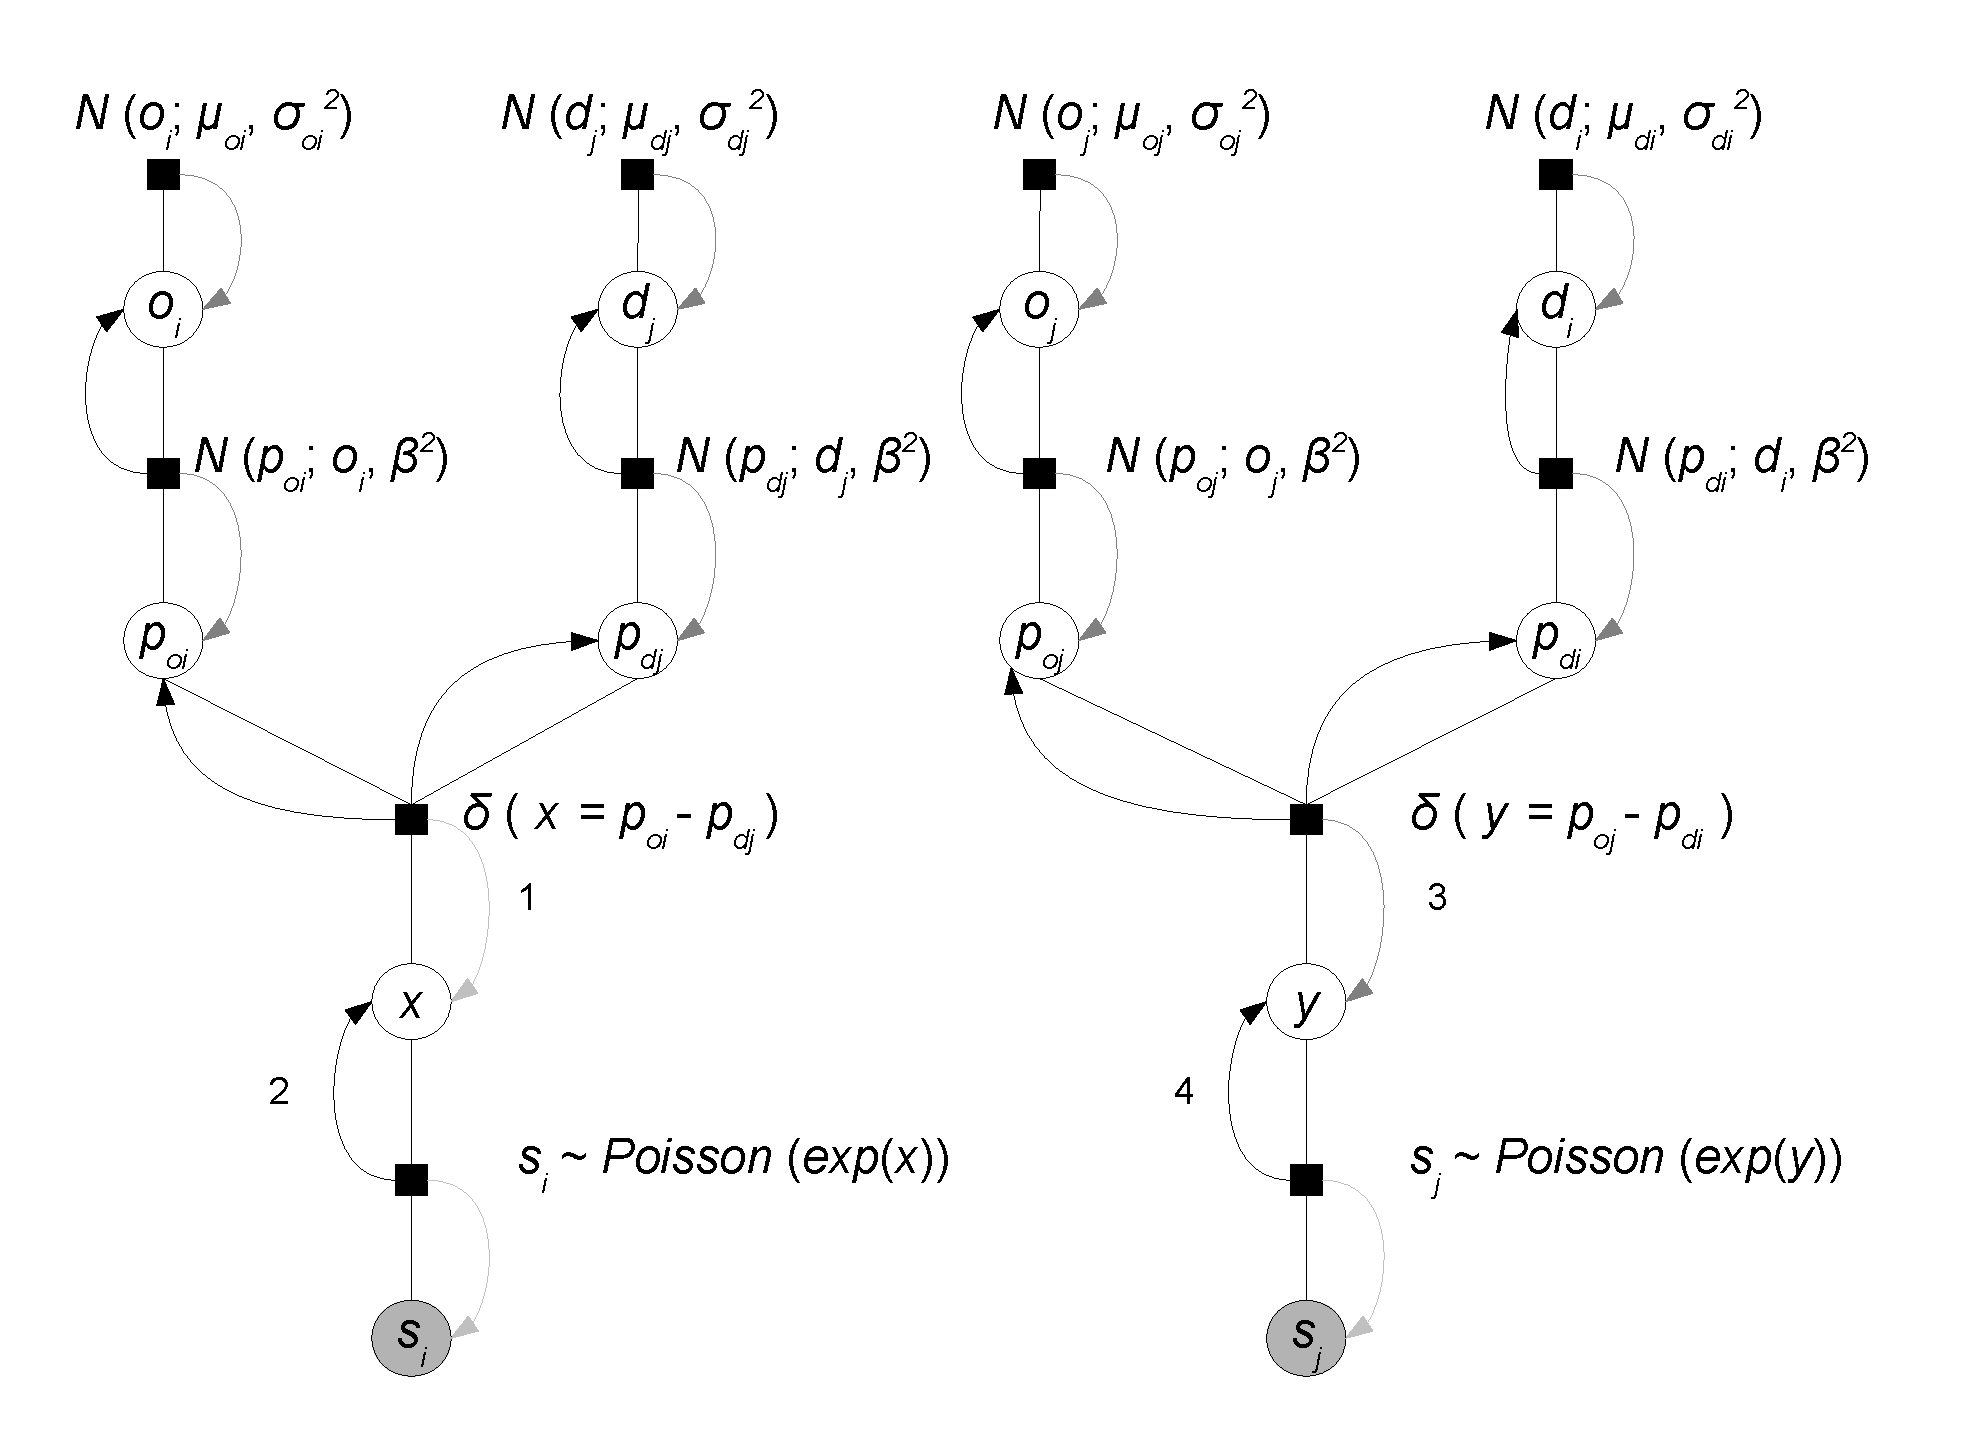
\includegraphics[scale=0.28]{modelAndInference}}
\caption{\small
The Poisson-OD (P) and Gaussian-OD (N) variants of TrueSkill factor graph for skill update of two teams based on the match score outcome (Left: modeling $s_i$; Right: modeling $s_j$). Note that the Poisson-OD and Gaussian-OD graphical models are merged due to limited space. Note also that the score observation factors use the Poisson distribution for the Poisson-OD model and the normal distribution for the Gaussian-OD model. The shaded variables are the observed ones. For each
team $i$, it is characterized by offence skill $o_{i}$ (the offence skill of team $i$) and defence skill $d_{i}$ (the defence skill of
team $i$). Given $s_j$ for team $j$, the posterior distributions over $(o_i,d_j)$ are inferred via message passing.
}
\label{fig:trueskill_variant}
\end{figure}
%%%%%%%%%%%%%%%%%%%%%%%%%%%%%%%%%%%%%%%%%%%%%%%%%%%%%%%%%%%%%%%

\subsubsection{Gaussian Offence/Defence Skill Model}

An alternative to the previous Poisson model is to
model $s_i \in \mathbb{R}$ and assume it
is generated as $s_{i}\sim \mathcal{N}(\mu, \gamma^2)$,
where $\mu = p_{oi}-p_{dj}$.  One can similarly
model $s_j$ by applying the same strategy when given $\mu = p_{oj} -
p_{di}$.  We note that unlike the Poisson model, $\mu$ can be negative
here so we need not exponentiate it.  While this allows us to directly
model match outcomes that allow negative team scores (c.f., Halo2 as
discussed in Section~\ref{sec:data_sets}), it is problematic for other
match outcomes that only allow non-negative team scores.  One
workaround would be to introduce a truncated Gaussian model to avoid
the problem of assigning non-zero probability to negative scores, but
we avoid this complication in exchange for the simple and exact
updates offered by a purely Gaussian model.

We show the resulting \emph{Gaussian-OD} model in
Figure~\ref{fig:trueskill_variant}(N), which
differs from our proposed Poisson model only in modeling the observed score $s_i$ ($s_j$) for team $i$ ($j$) given the univariate performance difference variable $x$ ($y$). In this model, all messages passed during inference
are Gaussian, allowing for efficient and exact belief updates.

%%%%%%%%%%%%%%%%%%%%%%%%%%%%%%%%%%%%%%%%%%%%%%%%%%%%%%%%%%%%%%
%\begin{figure}[htbp!]
%\vspace{-3mm}
%\centerline{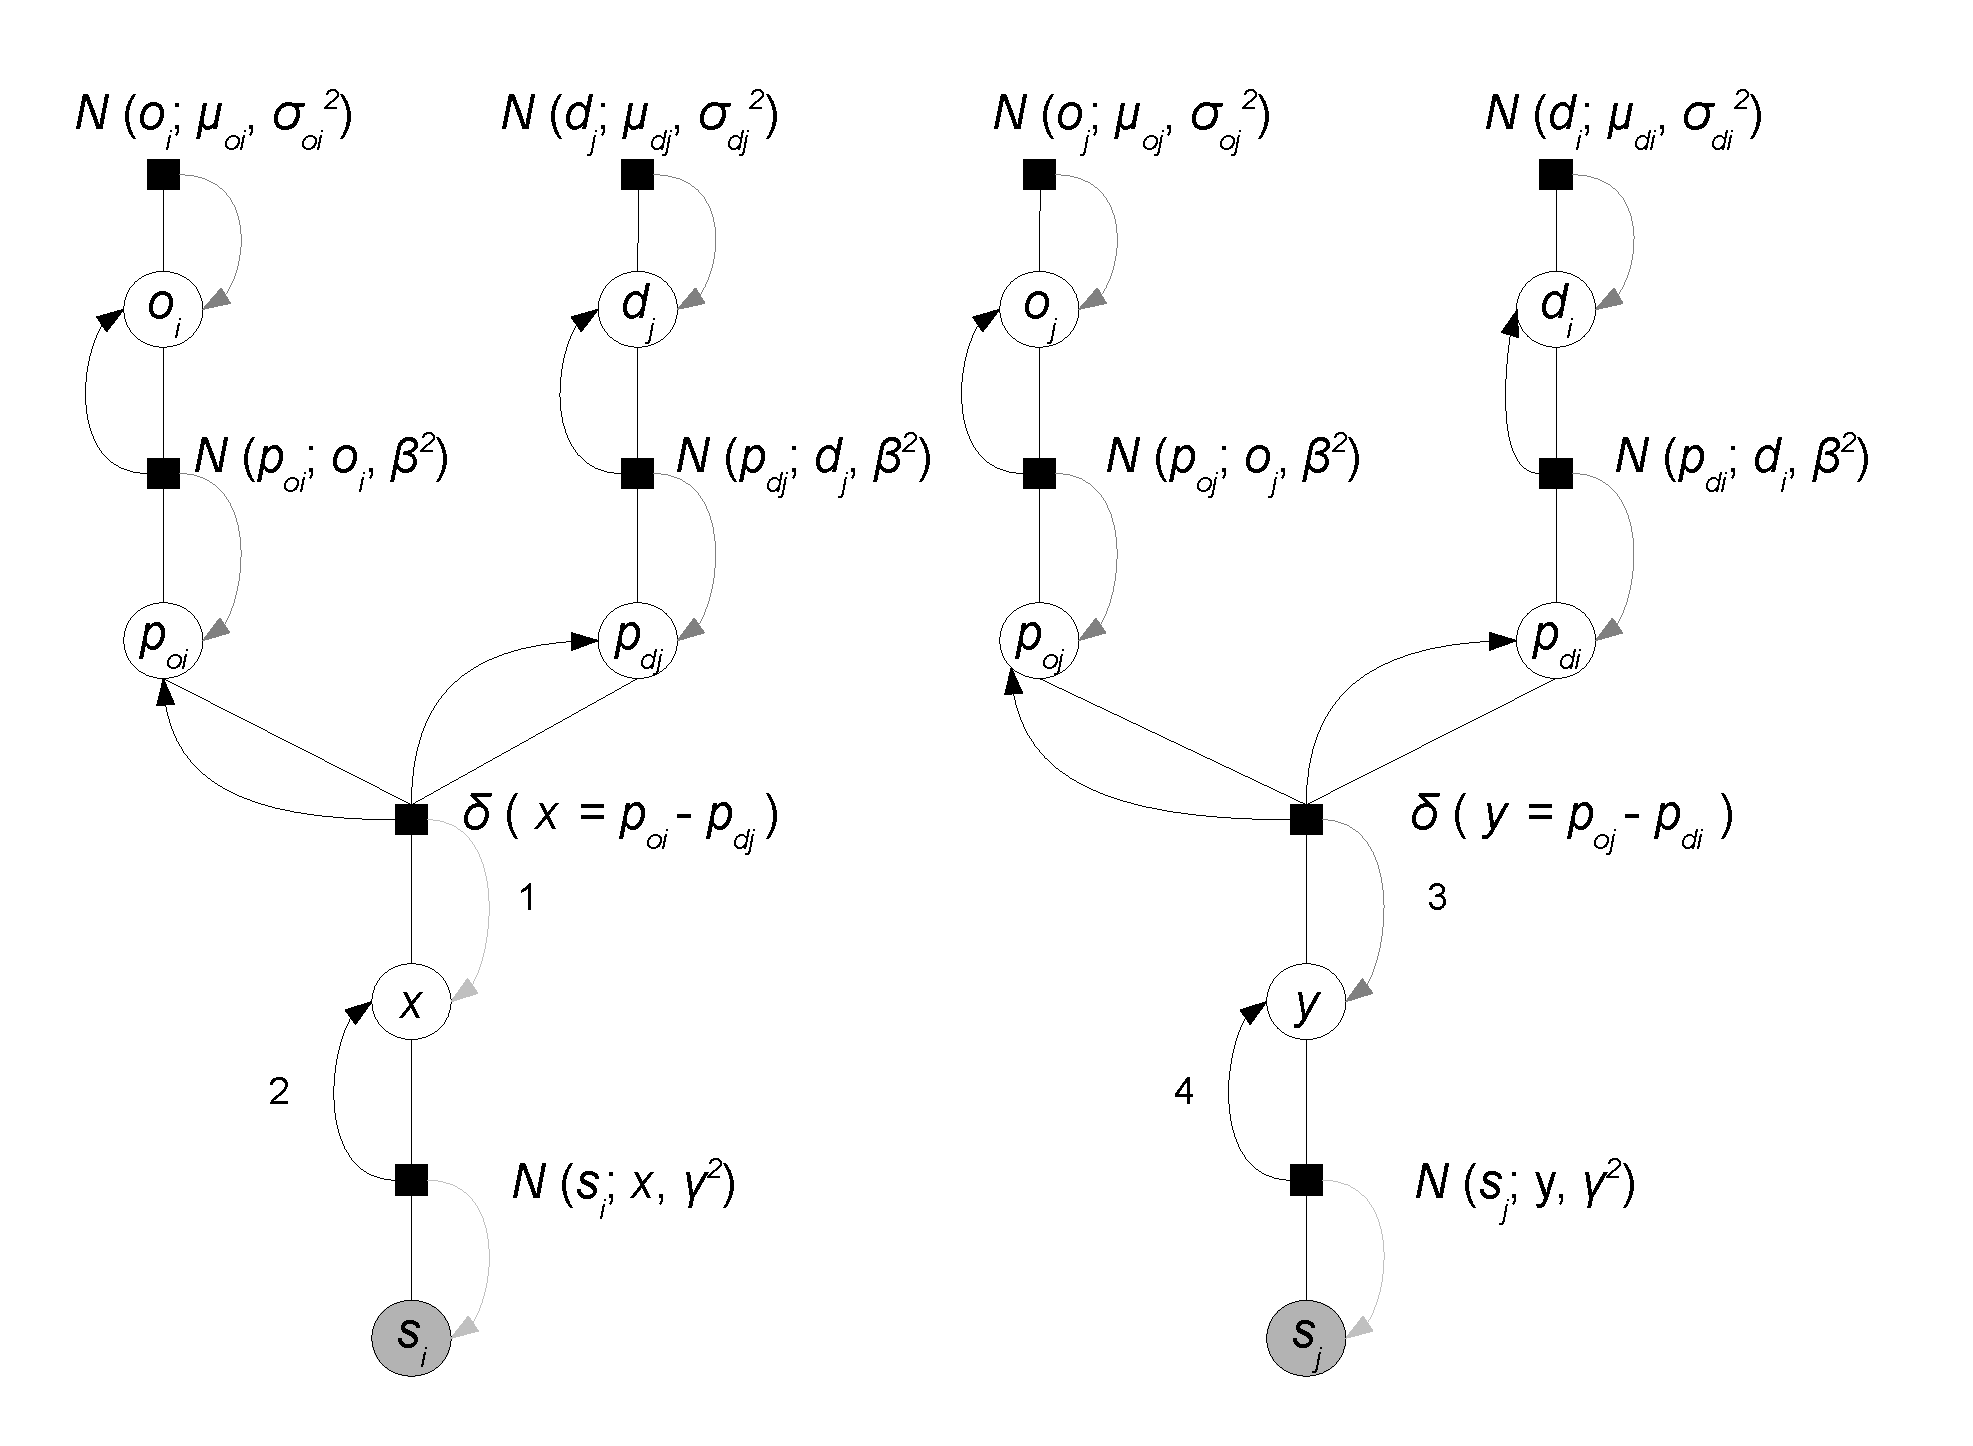
\includegraphics[scale=0.28]{modelAndInferenceGaussianGraphicalModel}}
%\vspace{-3mm}
%\caption{\small
%Gaussian-OD model for score-based skill learning (Left: modeling
%$s_i$; Right: modeling $s_j$). The shaded variables are the observed
%ones. Both team $i$ and team $j$ are characterized by offence skill
%$o_{i}$ (team $i$'s offence skill) and defence skill $d_{i}$ (team
%$i$'s defence skill). Given match outcomes $s_i$ and $s_j$, the
%posteriors over $o_i$ and $d_j$ can be exactly inferred using message
%passing.}
%\vspace{-2mm}
%\label{fig:modelAndInferenceGaussianGraphicalModel}
%\end{figure}
%%%%%%%%%%%%%%%%%%%%%%%%%%%%%%%%%%%%%%%%%%%%%%%%%%%%%%%%%%%%%%

\subsection{Gaussian Score Difference (SD) Model}

Again assuming $s_i \in \mathbb{R}$ and $s_j \in \mathbb{R}$,
algebra for the performance means in % the Gaussian offense/defense skill model
Figure~\ref{fig:trueskill_variant}(N) gives:
{\small\begin{align}
% Not sure this is it: \mu_{si} = o_i - d_j,    \;\;\;\;   \mu_{sj} = o_j - d_i.
%s_i = o_i - d_j,    \;\;\;\;   s_j = o_j - d_i.
s_i = p_{oi}-p_{dj}, \qquad \;\; s_j = p_{oj}-p_{di}.
\label{eq:ScoreDifferenceGaussianGraphicalModel}
\end{align}}
%where $\mu_{si}$ and $\mu_{sj}$ are the means for the Gaussian
%distributions of the score variables $s_i$ and $s_j$,
%respectively. \eqref{eq:ScoreDifferenceGaussianGraphicalModel}
This implies
{\small\begin{align}
  s_i - s_j &= (p_{oi} - p_{dj}) - (p_{oj} - p_{di})  \nonumber \\
            &= \underbrace{(p_{oi}+p_{di})}_{p_{li}} - \underbrace{(p_{oj}+p_{dj})}_{p_{lj}},
\end{align}}
\unindent which is like modeling the score difference with performance
expressions $p_{li}$ and $p_{lj}$ of respective univariate skill levels, $l_i$
and $l_j$.  Motivated by
\eqref{eq:ScoreDifferenceGaussianGraphicalModel}, we propose a score
difference (SD) Gaussian model that uses a likelihood model for the
observed difference $s := s_i - s_j$ specified as $s \sim
\mathcal{N}(p_{li} - p_{lj}, \gamma^2)$ as shown in
Figure~\ref{fig:modelAndInferenceGaussianGraphicalModelScoreDifference}.

%%%%%%%%%%%%%%%%%%%%%%%%%%%%%%%%%%%%%%%%%%%%%%%%%%%%%%%%%%%%%%%%%%%%%
\begin{figure}
\vspace{-0.5cm}
\centerline{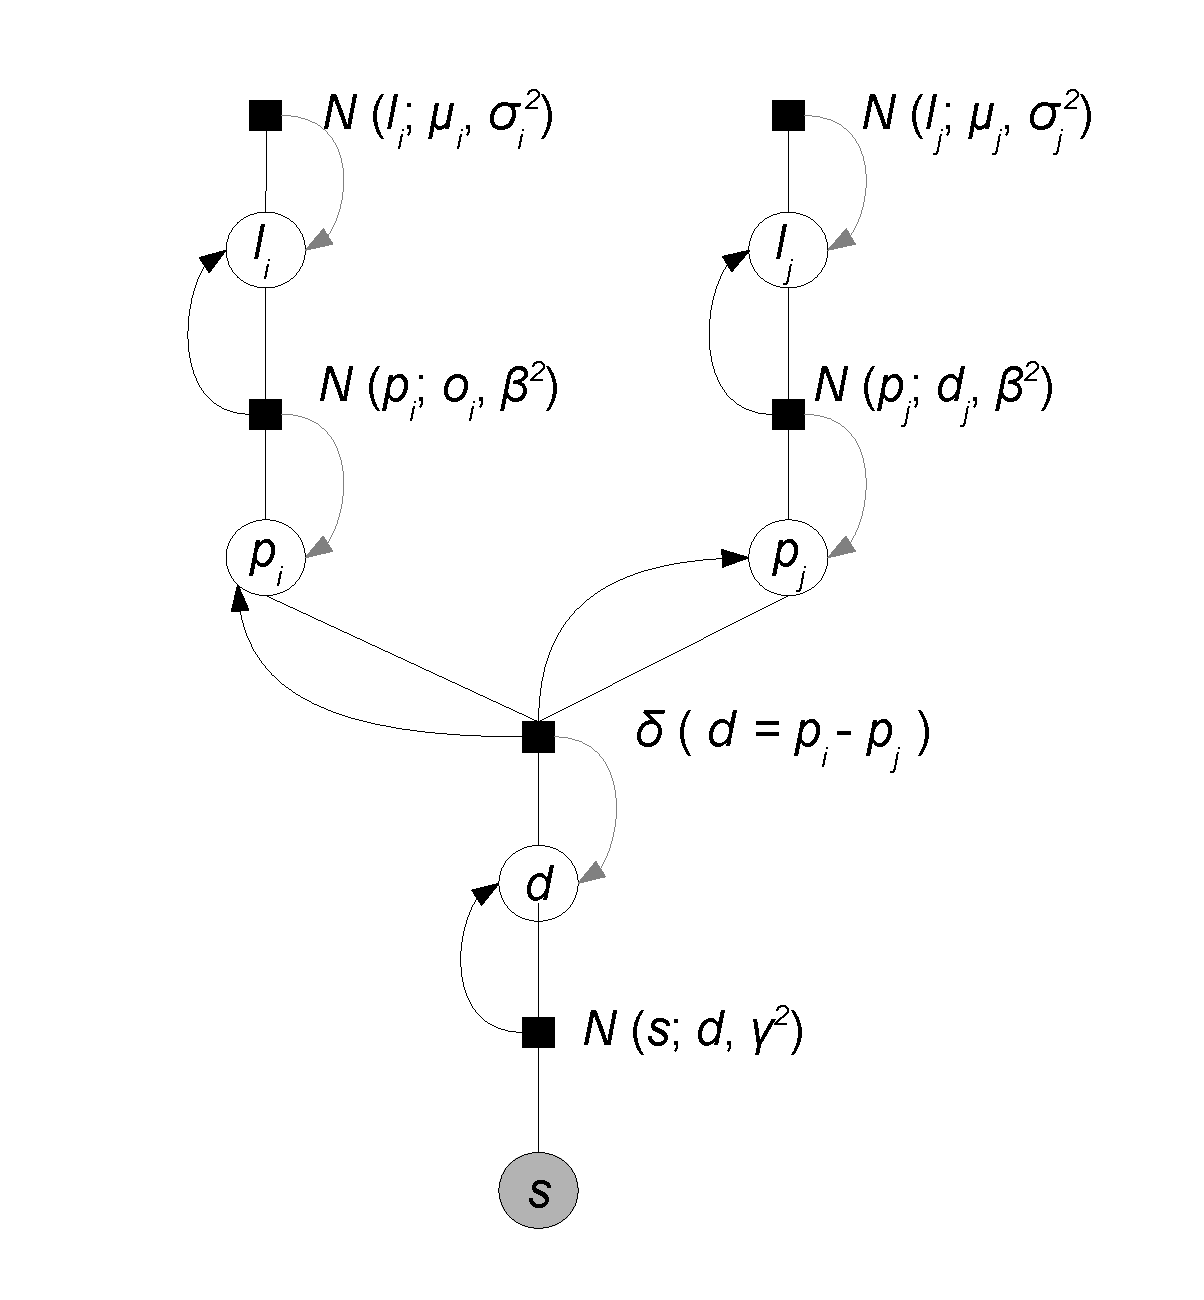
\includegraphics[scale=0.275]{modelAndInferenceGaussianGraphicalModelScoreDifference}}
\vspace{-3mm}
\caption{\small
Gaussian-SD model for skill learning from score differences.  Both team
$i$ and team $j$ are characterized by skill level $l_i$ and $l_j$,
respectively. The shaded variable $s$ ($s=s_i-s_j$) denotes the score
difference between $s_i$ and $s_j$. Bayesian inference for the posterior
skill level distributions has a closed-form solution.}
\label{fig:modelAndInferenceGaussianGraphicalModelScoreDifference}
\vspace{-2mm}
\end{figure}
%%%%%%%%%%%%%%%%%%%%%%%%%%%%%%%%%%%%%%%%%%%%%%%%%%%%%%%%%%%%%%%%%%%%%

\section{Skill and Win Probability Inference}

\label{sec:inference}

We infer skill distributions in all proposed models via
online Bayesian updating.  While exact inference in the purely Gaussian
models can be achieved by solving linear systems, Bayesian
updating provides an efficient (also exact) incremental learning alternative.
Equations for Bayesian updates and win probability inference are
model-dependent and presented below.

\subsection{Inference in TrueSkill}

\noindent{\bf Bayesian update:}
The Bayesian update equations in the TrueSkill model
(Figure~\ref{fig:trueskill}) are presented
in~\cite{herbrich06569}.

\noindent{\bf Win probability:} Given skill levels of
team $i$ and $j$, $l_i\sim\mathcal{N}(l_i;\mu_i,\sigma_i^2)$ and
$l_j\sim\mathcal{N}(l_j;\mu_j,\sigma_j^2)$, we first compute the
distribution over performance difference variable $d$, and get
$d\sim\mathcal{N}(d;\mu_d,\sigma_d^2)$ with $\mu_d = \mu_i - \mu_j$
and $\sigma_d^2 = \sigma_i^2 + \sigma_j^2+2\beta^2$. The winning
probability of team $i$ is given by the probability $p(d>0)$ defined as
{\small
\begin{align}
  p(d>0) = 1 - \Phi\left(\frac{-\mu_d}{\sigma_d}\right),
\end{align}}
where $\Phi(\cdot)$ is the normal CDF.

%{\bf Win probability:} Given skill levels of
%team $i$ and $j$, $l_i\sim\mathcal{N}(l_i;\mu_i,\sigma_i^2)$ and
%$l_j\sim\mathcal{N}(l_j;\mu_j,\sigma_j^2)$, we first compute the
%distribution over skill difference variable $d$, and get
%$d\sim\mathcal{N}(d;\mu_d,\sigma_d^2)$ with $\mu_d = \mu_i - \mu_j$
%and $\sigma_d^2 = \sigma_i^2 + \sigma_j^2$. The winning
%probability of team $i$ is given by transforming the skill difference with a logistic function as below
%\begin{align}
%  p(i\succ j) = E_{x\sim\mathcal{N}(d;\mu_d,\sigma_d^2)}\frac{1}{1+\exp(-x)},
%\label{eq:winProbDefinition}
%\end{align}
%
%The winning probability $p(i\succ j)$ defined above is the logistic-normal integral, and does not have an analytic form. We apply the results proposed in \cite{Maragakis08JCP} for approximation as below
%\begin{align}
%    p(i\succ j) \approx \frac{1}{1+\exp(-\gamma)}
%\end{align}
%where $\gamma = \sqrt{1+ \frac{\pi \sigma_d^2}{8}}$. Note that the absolute difference between approximation and the exact integral is always less than 0.02.

\subsection{Inference in Poisson-OD Model}
\label{sec:PoissonInference}

\noindent{\bf Bayesian update:}
Some of the update equations in the Poisson-OD model
(Figure~\ref{fig:trueskill_variant}(P)) have been presented in
\cite{herbrich06569}, with the exception of the marginal distribution
over $x$ and the message passing from the Poisson factor to $x$. Given
a prior Gaussian distribution over $x$, $\mathcal{N}(x;\mu,
\sigma^2)$, we next
demonstrate how to update the belief on $x$ when observing
team $i$'s score $s_i$.

By the sum-product algorithm \cite{kschischang01498}, the
marginal distribution of $x$ is given by a product of messages
{\small
\begin{align}\label{eq:marginal}
    p(x|s_i) = m_{\delta \rightarrow x}(x) m_{s_i \rightarrow x}(x).
\end{align}}
\unindent To avoid cluttered notation, let us use $m_1(x)$ to represent
$m_{\delta \rightarrow x}(x) = \mathcal{N}(x;\mu,\sigma^2)$, i.e., the message
passing from the factor $\delta(\cdot)$ to $x$, and $m_2(x)$ for
$m_{s_i\rightarrow x}(x) = Poisson(s_i;\exp(x))$, i.e.,
the message passing from the Poisson
factor to $x$ (c.f., messages labeled 1 and 2 in
Figure~\ref{fig:trueskill_variant}(P)). Due to the multiplication of
$m_{1}(x)$ and $m_{2}(x)$, the exact marginal distribution of
$p(x|s_i)$ is not Gaussian, which makes exact inference
intractable. To maintain a compact representation of offence and
defence skills, one can approximate $p(x|s_i)$ within a variational
Bayes framework by %, contrasted with expectation propagation, i.e., to
choosing a Gaussian distribution $q(x)^*:
\mathcal{N}(x;\mu_{\text{new}}, \sigma_{\text{new}}^2)$ that minimizes
the KL divergence between $p(x|s_i)$ and $q(x)$, i.e.,
{\small
\begin{align}\label{eq:marginal2}
    q(x)^* = \argmin_{q(x)} \text{KL}\left[q(x)|| p(x|s_i)\right].
\end{align}}
%where $\text{KL}[p(x)||q(x)]=\int p(x)\log \frac{p(x)}{q(x)}dx$.
We derive a fixed-point approach for optimizing $q(x)$ \cite{Beal:EMFixedPoint02} and describe this approach below.

%%%%%%%%%%%%%%%%%%%%%%%%%%%%%%%%%%%%%%%%%%%%%%%%%%%%%%%%%%%%%%%%%%%
\noindent{\bf Minimizer $q(x)$ for $\text{KL}(q(x)||p(x|s_i))$:}
We first expand the KL-divergence into its definition:
{\small
\begin{align}\label{eq:KL}
    \text{KL}\left(q(x)|| p(x|s_i)\right) &= \int q(x) \log \left( \frac{q(x)}{p(x|s_i)} \right) dx \nonumber \\
%    &= -\left(\underbrace{-\int q(x) \log (q(x)) d(x)}_{\text{entropy of }q(x)}\right) - \int q(x) \log \left( p(x|s_i) \right) dx \nonumber \\
     \qquad &= -\log\sqrt{2\pi e \sigma_{new}^2} - E_{x\sim q(x)} \log \left( p(x|s_i) \right),
\end{align}}
\unindentmore where $p(x|s_i)$ is the posterior probability of $x$ when
observing the score $s_i$. Since $q(x)$ is Gaussian
and the posterior has convenient Gaussian parts, manipulation of this
yields an equation for $\mu_{new}$ and $\sigma_{new}^2$ that can be
solved using an iterative fixed-point approach:
\begin{lemma}
Values for $\mu_{new}$ and $\sigma_{new}^2$
minimizing $\text{KL}\left(q(x)|| p(x|s_i)\right)$
satisfy
{\small
\begin{align}\label{eq:ExactMuSigmaNew}
    \mu_{\text{new}} & = \sigma^{2}\left(s_i - e^\kappa\right) + \mu, \nonumber \\
   \sigma_{\text{new}}^2 & = \frac{\sigma^2}{1+\sigma^2 e^\kappa },
\end{align}}
where
{\small
\begin{align}\label{eq:approximationZQuad5}
     \kappa  &= \log\left(\frac{\mu + s_i\sigma^2-1-\kappa+\sqrt{(\kappa - \mu - s_i\sigma^2 -1)^2+2\sigma^2}}{2\sigma^2}\right).
\end{align}}
\end{lemma}
\begin{proof}
The second term in~\eqref{eq:KL} is evaluated using
Bayes Theorem,
$p(x|s_i)=p(s_i|x)p(x)/p(s_i)$.
The term in $\log p(s_i)$ can be dropped because it is constant
with respect to $\mu_{\text{new}}$ and $\sigma_{\text{new}}^2$.
The term $E_{x\sim q(x)} [\log p(s_i|x)]$ is found by expanding the
Poisson distribution and noting $E_{x\sim p(x)}[\exp(x)] = \exp(\mu+\sigma^2/2)$ (see the Supplemental material\footnote{Available at \url{http://users.cecs.anu.edu.au/~sguo/sbsl_ecml2012_final_supple.pdf}} for derivation).
Thus it becomes
{\small
\begin{equation}\label{eq:firstTermFinal}
  s_i \mu_{\text{new}} - \exp(\mu_{\text{new}} + \sigma_{\text{new}}^2/2) - \log(s_i!)~.
\end{equation}}
\noindent
% Appendix \ref{app:exponentialIntegral} for derivation)
The term $E_{x\sim q(x)}[\log p(x)]$
according to the derivation in the Supplemental material
becomes
{\small
\begin{equation}\label{eq:finalSecondTerm}
     -\frac{1}{2}\log(2\pi\sigma^2) -
         \frac{1}{2\sigma^2}\left(\sigma_{new}^2 + \mu_{new}^2-2\mu\mu_{new} + \mu^2 \right)~.
\end{equation}}
Plugging~\eqref{eq:firstTermFinal} and~\eqref{eq:finalSecondTerm} into
\eqref{eq:KL} gives
{\small
\begin{align*}
    &\arg\min_{q(x)}\text{KL}\left(q(x)|| p(x|s_i)\right) \equiv \arg\min_{q(x)}-\log\sqrt{2\pi e \sigma_{new}^2} - \nonumber \\
    &\bigg( \underbrace{s_i \mu_{\text{new}} - \exp(\mu_{\text{new}} + \sigma_{\text{new}}^2/2) - \log(s_i!)}_{E_{x\sim q(x)} (\log p(s_i|x))} \nonumber \\ 
    & \underbrace{-\frac{1}{2}\log(2\pi\sigma^2) - \frac{1}{2\sigma^2}\left(\sigma_{new}^2 + \mu_{new}^2-2\mu\mu_{new} + \mu^2 \right)}_{E_{x\sim q(x)}(\log p(x))} \bigg).
\end{align*}}
To find the minimizer $q(x)$, we calculate the partial derivatives of
$\text{KL}\left(q(x)|| p(x|s_i)\right)$ w.r.t.\
$\mu_{\text{new}}$ and $\sigma_{new}$, and set them to zero, leading to% as below
%{\small
%\begin{align*}
%    \partial{(\text{KL}\left(q(x)|| p(x|s_i)\right))}{\partial{\mu_{\text{new}}}} & = -s_i + \exp(\mu_{\text{new}}+\frac{\sigma_{\text{new}}^2}{2}) + \frac{\mu_{\text{new}}-\mu}{\sigma^2}, \\
%    \frac{\partial(\text{KL}\left(q(x)|| p(x|s_i)\right))}{\partial{\sigma_{\text{new}}}} &= -\frac{1}{\sigma_{\text{new}}} + \sigma_{\text{new}} \exp(\mu_{\text{new}}+\frac{\sigma_{\text{new}}^2}{2})+ \frac{\sigma_{\text{new}}}{\sigma^2}.
%\end{align*}}
%
%Setting the right hand sides of both partial derivatives to $0$ gives
{\small
\begin{align}
    \mu_{\text{new}} & = \sigma^{2}\left(s_i - \exp\left(\mu_{\text{new}}+\frac{\sigma_{\text{new}}^2}{2}\right)\right) + \mu, \nonumber \\
   \sigma_{\text{new}}^2 & = \frac{\sigma^2}{1+\sigma^2 \exp(\mu_{\text{new}}+\frac{\sigma_{new}^2}{2})}~.\nonumber
\end{align}}
Summing the first plus half the second of these equations,
and defining $\kappa=\mu_{\text{new}}+\sigma_{\text{new}}^2/2$
yields the equation for $\kappa$ of
{\small
\begin{align}\label{eq:kappa}
    \kappa & = \mu + \sigma^2(s_i - \exp(\kappa)) + \frac{\sigma^2}{2(1+\sigma^2\exp(\kappa))},
\end{align}}
and one gets~\eqref{eq:ExactMuSigmaNew} in terms of $\kappa$.
%Note that the variance $\sigma_{\text{new}}^2$ does not explicitly depends on $s_i$.

We convert~\eqref{eq:kappa} by solving for $\exp(\kappa)$
as it appears on the right-hand side.  This yields
a quadratic equation, and we take the positive solution since $\exp(\kappa)$
must be non-negative (see the Supplemental material).
The result gives us~\eqref{eq:approximationZQuad5}.
\end{proof}

We can use~\eqref{eq:approximationZQuad5}
as a fixed-point rewrite rule.
For a given $\mu$ and $\sigma^2$ together with an initial value of
$\kappa$, one iterates~\eqref{eq:approximationZQuad5} until
convergence.  Empirically, this happens within 2-3 iterations.
With convergence, we substitute the fixed-point solution
into \eqref{eq:ExactMuSigmaNew} to get the optimal mean
and variance for $q(x)^*$.


%%%%%%%%%%%%%%%%%%%%%%%%%%%%%%%%%%%%%%%%%%%%%%%%%%%%%%%%%%%%%%%%%%%

%Let us directly present the result of optimizing $q(x)^*$ as below.
%(The derivation must be omitted due to space limitations.)
%% Detailed derivations can be found in Appendix~\ref{app:Minimizer}.
%The optimization consists of two steps. The first step is to iterate
%the following equation
%\begin{align}\label{eq:IterativeFixPoint}
%    z_{\text{new}}  =
%\log\left(\frac{\mu + s_i\sigma^2-1-z_{\text{old}}+\sqrt{(z_{\text{old}} - \mu - s_i\sigma^2 -1)^2+2\sigma^2}}{2\sigma^2}\right),
%\end{align}
%%%%%%%%%%%%%% Check "dimension" of the iteration: log(a/a^2) == log (1/a)
%with $\mu$, $\sigma^2$, and $s_i$ as defined in the messages above and
%where $z_{\text{old}}$ can be initialized with $\mu+\sigma^2/2$. The
%objective of iteration is to find a convergent $z^*$. The second step
%makes use of the $z^*$ found in the first step to estimate the
%Gaussian minimizer $q(x)^*$ with its mean and variance given as
%follows:
%\begin{align}\label{eq:ExactMuNew}
%    \mu_{\text{new}}  = \sigma^{2}\left(k_i - \exp(z^*)\right) + \mu, \;\;\;
%    \sigma_{\text{new}}^2  = \frac{\sigma^2}{1+\sigma^2 \exp(z^*)}.
%\end{align}
%Setting $p(x|s_i) :=
%\mathcal{N}(x;\mu_{\text{new}},\sigma_{\text{new}}^2)$, the remaining
%message passing to compute the posterior involves only Gaussians and
%can be done exactly and efficiently.

\noindent{\bf Win probability:}
Suppose we
are given the offence and defence skills for team $i$ and $j$, we can
estimate the distributions over performance difference variables of
$x$ and $y$ (c.f., Figure~\ref{fig:trueskill_variant}), and compute
the Poisson parameters for $s_i$ and $s_j$ by using $\lambda_i =
\exp(x)$ and $\lambda_j = \exp(y)$. To compute the winning probability
of team $i$, i.e., $p(s_i>s_j)$, we first construct a new variable $s
= s_i-s_j$, the difference variable between two Poisson distributions,
which proves to be a Skellam distribution in
\cite{Skellam46TheFrequencyDistribution}. Thus, we can compute the win
probability of $P(s>0)$ of team $i$, according to the probability mass
function for the Skellam distribution
{\small
\begin{align*}
     P(s=k; \lambda_i, \lambda_j) =e^{-(\lambda_i+\lambda_j)}\left(\frac{\lambda_i}{\lambda_j}\right)^{k/2}I_{|k|}\left(2\sqrt{\lambda_i\lambda_j}\right),
\end{align*}}
where $I_{k}(z)$ is the modified Bessel function of the first kind given in \cite{Abramowitz74HandbookOfMathematical}.
%{\small
%\begin{align}
%    I_k{(z)} = \left(\frac{z}{2}\right)^k\sum_{i=0}^{+\infty}\frac{(z^2/4)^i}{i!\Gamma(k+i+1)}.
%\end{align}}
We approximated $P(s>0,\lambda_i, \lambda_j)$ with
$\sum_{k=1}^{n} P(s=k; \lambda_i, \lambda_j)$ using $n=100$ since
$P(s=k; \lambda_i, \lambda_j) \approx 0$ for all of our experiments
when $k>100$.

%Suppose we are given the offence and defence skills (e.g., $o_i, d_i, o_j, d_j$) for team $i$ and $j$, we first represent a team's overall skill variable as the sum of its offence and defence skills, and then construct the skill difference variable for computing winning probability. More specifically, the skill difference $d$ between team $i$ and team $j$ is also a Gaussian distributed variable with its mean $\mu_{oi}+\mu_{di} - \mu_{oj}-\mu_{dj}$ and variance $\sigma_{oi}^2+\sigma_{di}^2 + \sigma_{oj}^2+\sigma_{dj}^2$. Given the distribution of this skill difference variable, one can apply \eqref{eq:winProbDefinition} in computing the winning probability.

\subsection{Inference in Gaussian-OD Model}

\noindent{\bf Bayesian update:} In the Gaussian-OD model
(Figure~\ref{fig:trueskill_variant}(N)), all
messages are Gaussian so one can
compute the belief update in closed-form as follows
{\small
\begin{align}
\label{eq:GaussianGraphicalModelsUpdatingEquation}
  \pi_{o_{i}}  =    \frac{1}{\sigma_{o_{i}}^2} + \frac{1}{\beta_1^2+\beta_2^2+\gamma^2+\sigma_{d_{j}}^2}, \qquad \tau_{o_{i}}    &=    \frac{\mu_{o_{i}}}{\sigma_{o_{i}}^2} + \frac{s_i+\mu_{d_{j}}}{\beta_1^2+\beta_2^2+\gamma^2+\sigma_{d_{j}}^2},  \nonumber \\
  \pi_{d_{j}}  =    \frac{1}{\sigma_{d_{j}}^2} + \frac{1}{\beta_1^2+\beta_2^2+\gamma^2+\sigma_{o_{i}}^2}, \qquad \tau_{d_{j}}    &=    \frac{\mu_{d_{j}}}{\sigma_{d_{j}}^2} + \frac{\mu_{o_{i}}-s_i}{\beta_1^2+\beta_2^2+\gamma^2+\sigma_{o_{i}}^2},
\end{align}}
\unindentmore where $\mu_{o_{i}}$ and $\sigma_{o_{i}}$ are the mean
and standard deviation of the prior offence skill distribution of team
$i$, $\pi_{o_{i}} (\pi_{d_{j}}) = \frac{1}{\sigma_{\mathit{post}}^2}$
and $\tau_{o_{i}} (\tau_{d_{j}}) =
\frac{\mu_{\mathit{post}}}{\sigma_{\mathit{post}}^2}$ are the
precision and precision-adjusted mean for the posterior offence
(defence) skill distribution of team $i$ ($j$).  Likewise, one can
derive the update equations for team $j$'s offence skill $o_j$ and
team $i$'s defence skill $d_i$.

\noindent{\bf Win probability:} To compute
the probability of team $i$ winning vs team $j$, we first use message
passing to estimate the normally distributed distributions for score
variables $s_i$ and $s_j$, and then compute the probability that
$s_i-s_j>0$, i.e., team $i$'s score is larger than team $j$'s. Given
$s_i\sim\mathcal{N}(s_i;\mu_{si},\sigma_{si}^2)$ and
$s_j\sim\mathcal{N}(s_j;\mu_{sj},\sigma_{sj}^2)$, we can compute the
winning probability of team $i$ by
\begin{align}
  p(s>0) = 1 - \Phi\left(\frac{-(\mu_{si}-\mu_{sj})}{\sigma_{si}^2+\sigma_{sj}^2}\right).
\end{align}
%TODO: how about the draw probability in Gaussian models?
%Does Gaussian ever predict draw?

\subsection{Inference in Gaussian-SD Model}

\noindent{\bf Bayesian update:} In the Gaussian-SD model
(Figure~\ref{fig:modelAndInferenceGaussianGraphicalModelScoreDifference}),
all messages are Gaussian so we can again derive the update
for the single team skills $l_i$ and $l_j$ in closed-form
as follows:
{\small
\begin{align}
%\label{eq:GaussianGraphicalModelsUpdatingEquation}
  \pi_{l_{i}}  =  \frac{1}{\sigma_{l_{i}}^2} + \frac{1}{\beta_1^2+\beta_2^2+\gamma^2+\sigma_{l_{j}}^2}, \qquad  \tau_{l_{i}} =    \frac{\mu_{l_{i}}}{\sigma_{l_{i}}^2} + \frac{(s_i-s_j)+\mu_{l_{j}}}{\beta_1^2+\beta_2^2+\gamma^2+\sigma_{l_{j}}^2},                                      \\
  \pi_{l_{j}}  =    \frac{1}{\sigma_{l_{j}}^2} + \frac{1}{\beta_1^2+\beta_2^2+\gamma^2+\sigma_{l_{i}}^2}, \qquad \tau_{l_{j}} =    \frac{\mu_{l_{j}}}{\sigma_{l_{j}}^2} + \frac{\mu_{l_{i}}-(s_i-s_j)}{\beta_1^2+\beta_2^2+\gamma^2+\sigma_{l_{i}}^2},
  \end{align}}
where $\mu_{l_i}$ ($\mu_{l_j}$) and $\sigma_{l_i}$
      ($\sigma_{l_j}$) are the mean and standard deviation of team
      $i$'s (team $j$'s) prior skill distribution,
    % \item
$\pi_{l_{i}}$ ($\pi_{l_{j}}$) and $\tau_{l_{i}}$
      ($\tau_{l_{j}}$) are the precision and precision adjusted mean
      for team $i$'s (team $j$'s) posterior skill distribution.
    % \item $\mu_{l_j}$ and $\sigma_{l_j}$ are the mean and standard deviation of team $j$'s prior skill distribution,
    % \item $\pi_{l_{j}}$ and $\tau_{l_{j}}$ are the precision and precision adjusted mean for team $j$'s posterior skill distribution.
%\end{itemize}

\noindent{\bf Win probability:} To estimate the winning probability of team $i$ for a match with team $j$, one can first use message passing to estimate the normally distributed score difference variable $s$, and then compute the winning probability of team $i$ by
{\small
\begin{align}
  p(s>0) = 1 -
  \Phi\left(\frac{l_i-l_j}{\sigma_i^2+\sigma_j^2+2 \beta^2}\right),
\end{align}}
where $l_i$ and $\sigma_i$ are the mean and standard deviation for
team $i$'s skill level, and $\beta$ the standard deviation of the
performance variable.

%To estimate the winning probability of team $i$ for a match with team $j$, one can first use message passing to estimate the normally distributed score difference variable $s$, and then compute the winning probability of team $i$ by
%{\small
%\begin{align}
%  p(s>0) = 1 -
%  \Phi\left(\frac{l_i-l_j}{\sigma_i^2+\sigma_j^2+2 \beta^2}\right),
%\end{align}}
%where $l_i$ and $\sigma_i$ are the mean and standard deviation for
%team $i$'s skill level, and $\beta$ the standard deviation of the
%performance variable.

\section{Empirical Evaluation}

\subsection{Data Sets}

\label{sec:data_sets}

Experimental evaluations are conducted on three data sets: Halo 2 XBox Live
matches, Australian Football
(Rugby) League (AFL)%\footnote{\noindent
%  \url{http://www.csse.monash.edu.au/~footy/data/index.shtml}}
and UK
Premier League (UK-PL)\footnote{\noindent \url{http://www.football-data.co.uk/englandm.php}}.  The Halo 2 data consists of a
set of match outcomes comprising 6227 games for 1672 players. We note there are negative scores for this data, so we add the absolute value of the minimal score to all scores to use the data with all proposed models.

The training and testing settings are described as follows.  For Halo
2~\footnote{\noindent Credit for the use of the Halo 2 Beta Data set
is given to Microsoft Research Ltd. and Bungie.}, the last 10\%
of matches are used for testing, and we use different proportions of
the first 90\% of data for training. There are 8 proportions used
for training, ranging from 10\% to 80\% with an increment of
10\%, and 90\% is not used for training due to cross validation. To cross validate, we sample the data and run the learning 20 times at each proportion level
to get standard error bars. Note that there are some players in the
testing games who are not involved in any training data sets,
particularly when small proportion of training data set is selected
(e.g., the first 10 percent games); we remove these games in the
testing set when reporting performances for all models.

%The training and testing settings are described as follows.  For Halo
%2~\footnote{\noindent Credit for the use of the Halo 2 Beta Data set
%is given to Microsoft Research Ltd. and Bungie.}, the last 20\%
%of matches are used for testing, and we use different proportions of
%the first 80\% of data for training. There are 8 proportions used
%for training, ranging from 10\% to 80\% with an increment of
%10\%. To cross validate, we
%sample the data and run the learning 30 times at each proportion level
%to get standard error bars. Note that there are some players in the
%testing games who are not involved in any training data sets,
%particularly when small proportion of training data set is selected
%(e.g., the first 10 percent games); we remove these games in the
%testing set when reporting performances for all models.


For both UK-PL and AFL datasets, cross validation is performed by
training and testing for each year separately (14 years for UK-PL, and
11 years for AFL).  For these two datasets, we test the last 20\%
percent of matches in each year, with the training data increasing
incrementally from 10\% to 80\% of the initial matches.

\subsection{Evaluation Criteria}

%We evaluate performances using three criteria: {\it information gain}
%of predicting winning probability of a team
%(Section~\ref{sec:informationGain}),
%{\it win/lose prediction accuracy}
%(Section~\ref{sec:WLPredictionAccuracy}),
%and {\it score prediction errors}
%(Section~\ref{sec:scorePredictionError}).
%While the first two criteria focus on predicting win/lose, the third
%criterion measures how good a model is at predicting scores, for which
%TrueSkill does not apply since it is restricted to WLD only. Let us
%introduce each criterion in detail.

\subsubsection{Information Gain}
\label{sec:informationGain}

The first criterion we use to evaluate different approaches is
\emph{information gain}, which is proposed in the \emph{Probabilistic Footy
Tipping Competition}\footnote{Refer to
\url{http://www.csse.monash.edu.au/~footy/}}: if a predictor assigns
probability $p$ to team $i$ winning, then the score (in ``bits")
gained is $1+\log_2(p)$ if team $i$ wins, $1+\log_2(1-p)$ if team $i$ loses, $1+(1/2)\log_2(p(1-p))$ if draw happens.
%This evaluation metric can be viewed as an information gain
%interpretable variant of a log likelihood score where an uninformed
%prediction of $p=0.5$ leads to a score of 0 and a definite prediction
%of $p=1$ ($p=0$) leads to a score of $-\infty$ if predicting
%incorrectly and 1 if predicting correctly.
In Section~\ref{sec:inference}, we showed how to compute the win
probability $p$ for each model.

\subsubsection{Win/no-Win Prediction Accuracy}
\label{sec:WLPredictionAccuracy}

While information gain provides a sense of how well the models fit the
data, it is also interesting to see how accurate the models were at
predicting match outcomes in terms of win/no-win (e.g., loss/draw).  To compare
classification performance of each model, we report the
win/not winning prediction accuracy in terms of area under the curve (AUC) for the
games with a win or loss outcome.

%This is a straighforward metric to
%evaluate in expectation: for the univariate skill models we simply
%assign a win to the team with the higher mean skill level, for the
%remaining offence/defence score models, we simply assign a win to the
%team with the higher expected score (these simple calculations are
%explained in the next subsection).

%It is essential to evaluate the prediction accuracy in terms of
%win/loss for matchmaking. To describe this evaluation criterion, let
%us first introduce when a model predicts team $i$ winning, in a match
%with team $j$. Based on the belief of a model, its prediction is
%correct: either (1) team $i$'s mean skill is larger than that of team
%$j$ skill and team $i$ wins, or (2) team $i$'s mean skill is smaller
%than that of team $j$ skill and team $i$ loses. Suppose there are $M$
%matches, and the model predicts correctly for $N$ times, then the
%prediction accuracy is $N/M$.

\subsubsection{Score Prediction Error}
\label{sec:scorePredictionError}

%We evaluate the score prediction accuracy for the two full
% score prediction models: Poisson-OD and Gaussian-OD.
%For the Poisson-OD model (Figure~\ref{fig:trueskill_variant}), the
%expected score for team $i$ ($j$) is $\exp(x)$ ($\exp(y)$) and for the
%Gaussian-OD model
%(Figure~\ref{fig:modelAndInferenceGaussianGraphicalModel}), the
%expected score for team $i$ ($j$) is $x$ ($y$), where $x$ ($y$) is the
%difference in mean performances giving $s_i$ ($s_j$).  The Gaussian-SD model
%(Figure~\ref{fig:modelAndInferenceGaussianGraphicalModelScoreDifference}),
%directly produces \emph{score difference} predictions $d = s_i - s_j$,
%which is just the difference in mean performances of the two teams.
%Because scores for different games have a different scale, we introduce
%a relative measure of score accuracy.
%Suppose $s^*$ is the true score, and
%$\hat{s}$ the expected score. We define the
%relative score prediction error $e(s^*, \hat{s})$ as
%\begin{align}
%e(s^*, \hat{s})= \frac{|\hat{s}-s^*|}{|s^*|}.
%\end{align}
%%Therefore, the larger the deviation of $\hat{s}$ to the true score $s^*$, the larger the error.
%Note that the prediction error can be larger than one,
%e.g. $\hat{s}=5, s^*=2$ causing $e(s^*, \hat{s})=1.5$.




%For the Poisson-OD model (Figure~\ref{fig:trueskill_variant}), the
%expected score for team $i$ ($j$) is $\exp(x)$ ($\exp(y)$) and for the
%Gaussian-OD model
%(Figure~\ref{fig:modelAndInferenceGaussianGraphicalModel}), the
%expected score for team $i$ ($j$) is $x$ ($y$), where $x$ ($y$) is the
%difference in mean performances giving $s_i$ ($s_j$).  The Gaussian-SD model
%(Figure~\ref{fig:modelAndInferenceGaussianGraphicalModelScoreDifference}),
%directly produces \emph{score difference} predictions $d = s_i - s_j$,
%which is just the difference in mean performances of the two teams.
We evaluate the score prediction accuracy for Poisson-OD and
Gaussian-OD models for \emph{each} team in terms of the mean absolute
error (MAE). Note that we must omit the Gaussian-SD model since it can only
predict score differences rather than scores.

%, defined as below:
%{\small\begin{align}
%    \text{MAE} = \frac{1}{n} \sum_{i=1}^{2*n} | \hat{s_i} - s_i |
%\end{align}}
%where $\hat{s_i}$ is the predicted score, $s_i$ the ground truth, and $n$ the number of matches for matches involving two players.

%The MAE for the Gaussian-SD model is given as below.
%\begin{align}
%    \text{MAE} = \frac{1}{n} \sum_{i=1}^{n} | \hat{\text{sd}_i} - \text{sd}_i |
%\end{align}
%where $\hat{\text{sd}_i}$ is the predicted score difference for match $i$, and $\text{sd}_i$ is the ground truth for the score difference of match $i$.

%Denoted by $\text{SD}_{\text{predict}}$ and $\text{SD}_{\text{accuracy}}$
%respectively the {\it score
%difference} of a match based on models and ground truth data, we define the
%relative score prediction error $e(\text{SD}_{\text{predict}}, \text{SD}_{\text{accuracy}})$ as
%\begin{align}
% e(\text{SD}_{\text{predict}}, \text{SD}_{\text{accuracy}})=
% |\text{SD}_{\text{predict}} - \text{SD}_{\text{accuracy}}|.
%\end{align}

% \subsection{Logistic Regression}
% Perhaps the simplest score prediction approach is to use a linear regression model for $m$ teams and $n$ matches with variables $o_1,\ldots,o_m$ and $d_1,\ldots,d_m$
% can be setup as in the following example:
% \begin{equation*}
%     \underbrace{\begin{pmatrix}
%         1 & 0 & 0 & -1 & \dots & 0 & 0 \\
%         0 & -1 & 1 & 0 & \dots & 0 & 0 \\
%         0 & -1  & 0 & 0 & \dots & 1 & 0 \\
%         1 & 0  & 0 & 0 & \dots & 0 & -1 \\
%         \hdotsfor{7}                   \\
%         0 & 0  & 1 & 0 & \dots & 0 & -1\\
%         0 & 0  & 0 & -1 & \dots& 1 & 0
%     \end{pmatrix}}_{A}
%     \underbrace{\begin{pmatrix}
%         o_1 \\
%         d_1 \\
%         o_2 \\
%         d_2 \\
%         \hdotsfor{1} \\
%         o_m \\
%         d_m
%     \end{pmatrix}}_{\vec{z}}
%     =
%     \underbrace{\begin{pmatrix}
%         s_{1,1} \\
%         s_{1,2} \\
%         s_{2,m} \\
%         s_{2,1} \\
%         \hdotsfor{1} \\
%         s_{n,2} \\
%         s_{n,m}
%     \end{pmatrix}}_{\vec{s}},
% \end{equation*}
% where $s_{k,j},k=1,\dots,n$ is the team $j$'s score for the $k$th match. In order to use a logistic model, we propose mapping from $s_{kj},k=\{1,\dots,n\}$ to $t_{jk}$ by
% \begin{align*}
%     t_{jk} = \frac{1}{1+\exp(-s_{jk})}.
% \end{align*}
% Now the objective is to find the optimal skill vector $z^*$ defined as
% \begin{align*}
%     z^* = \arg\min_{z}||Az-\vec{t}||_{2}^2,
% \end{align*}
% which can be achieved by using maximum likelihood parameter estimation.


\subsection{Results}

\label{sec:results}

Experimental results are reported according to the parameter
configurations shown in Table~\ref{table:Parameters}. All results are
presented in Figure~\ref{fig:Results} and discussed below.
%\begin{table}
%\vspace{-5mm}
%\caption{Parameter settings. Priors on offence/defence skills: $\mathcal{N}(\mu_{0},\sigma_{0}^2)$ with $\mu_{0}=25$ and $\sigma_{0}=25/3$. Performance variance: $\beta$, $\beta_1$, $\beta_2$.}
%\begin{center}
%\small
%\begin{tabular}{|c|c|}
%  \hline
%  Model             & Parameter ($\epsilon,\gamma$ empirically estimated)\\
%  \hline
%  TrueSkill          & $\beta=\sigma_{0}/2$; \\
%                          & $\epsilon$: draw probability of datasets\\
%\hline
%  Poisson-OD         & $\beta_1=\beta_2=\sigma_{0}/2$\\
%\hline
%  Gaussian-OD    & $\beta_1=\beta_2=\sigma_{0}/2$;\\
%                         & $\gamma$: score variance in datasets\\
%\hline
%  Gaussian-SD & $\beta=\sigma_{0}/2$;  \\
%                        & $\gamma$: score difference variance in datasets\\
%  \hline
%\end{tabular}
%\label{table:Parameters}
%\end{center}
%\vspace{-5mm}
%\end{table}
{\small\begin{table}[htbp!]
\vspace{-5mm}
\caption{Parameter settings. Priors on offence/defence skills: $\mathcal{N}(\mu_{0},\sigma_{0}^2)$ with $\mu_{0}=25$ and $\sigma_{0}=25/3$. Performance variance: $\beta$, $\beta_o$, $\beta_d$.}
\begin{center}
\small
\begin{tabular}{cc}
  \hline
  Model             & Parameter ($\epsilon,\gamma$ empirically estimated)\\
  \hline
  TrueSkill          & $\beta=\sigma_{0}/2$, $\epsilon$: draw probability\\
  Poisson-OD         & $\beta_o=\beta_d=\sigma_{0}/2$\\
  Gaussian-OD    & $\beta_o=\beta_d=\sigma_{0}/2$, $\gamma$: score variance\\
  Gaussian-SD & $\beta=\sigma_{0}/2$, $\gamma$: score difference variance\\
  \hline
\end{tabular}
\label{table:Parameters}
\end{center}
\vspace{-5mm}
\end{table}}

%%%%%%%%%%%%%%%%%%%%%%%%%%%%%%%%%%%%%%%%%%%%%%%%%%%%%%%%%%%%%%%%%
\begin{center}
\begin{figure*}[t!]
 \centering
 \subfigure{
   \hspace{-1.2cm}
   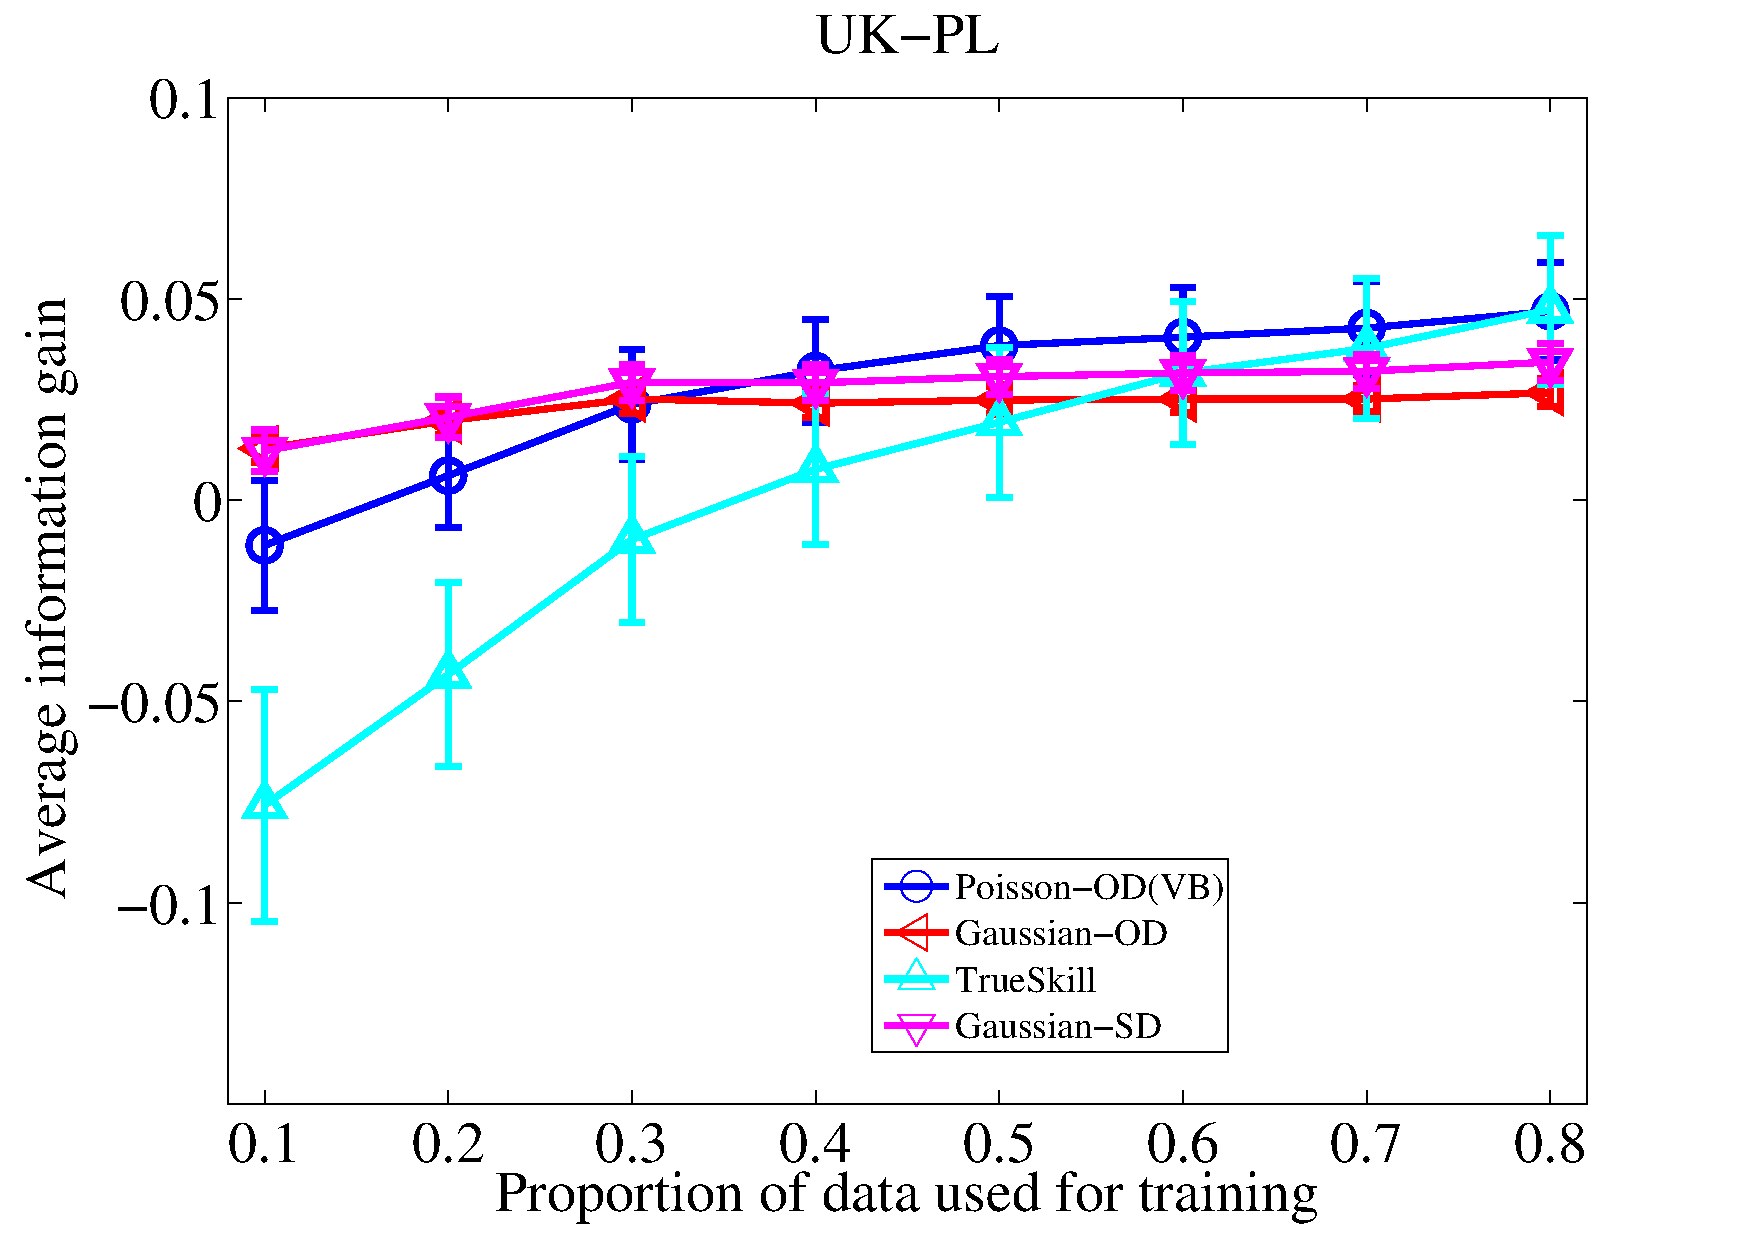
\epsfig{file=InforGain_UK, angle=0, height=3.6cm}
   \hspace{-0.725cm}
   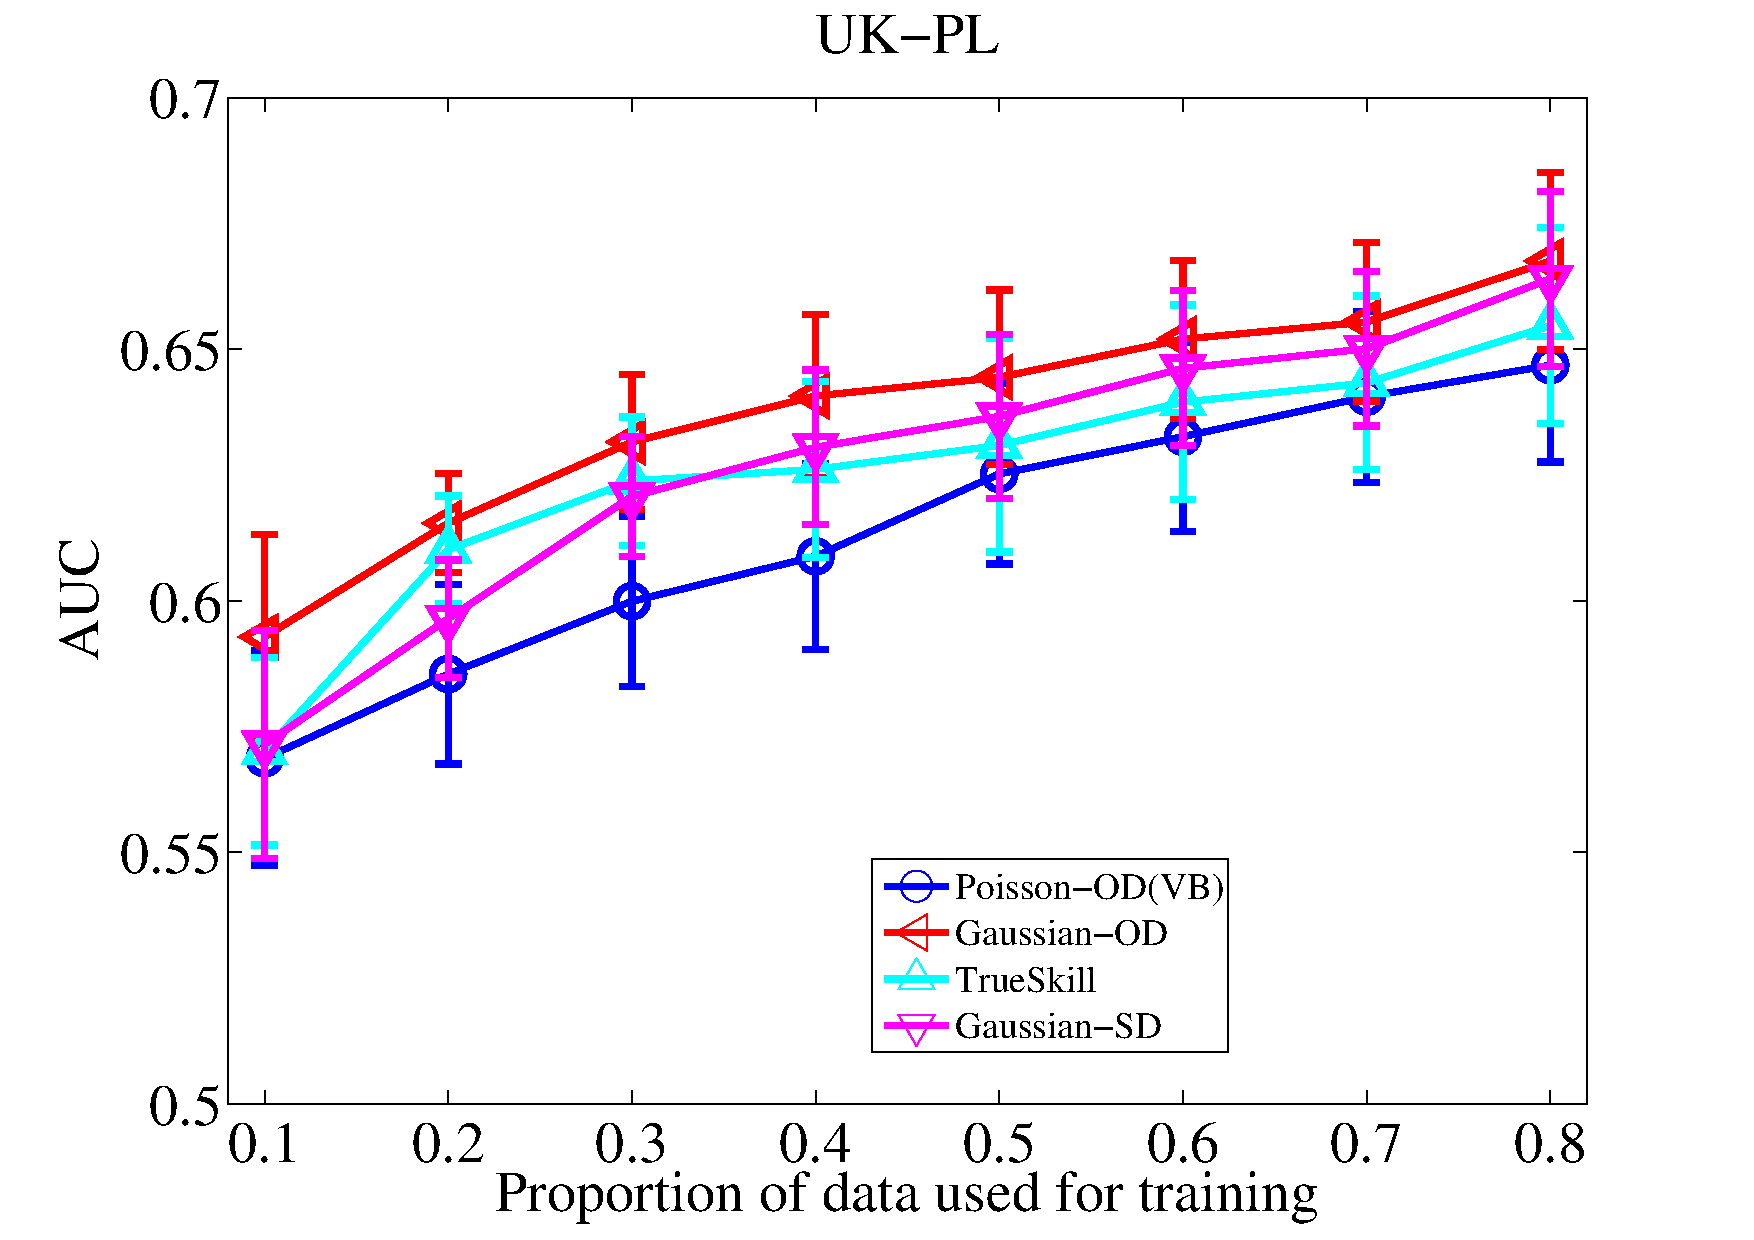
\epsfig{file=WLAccuracy_UK, angle=0, height=3.6cm}
   \hspace{-0.725cm}
   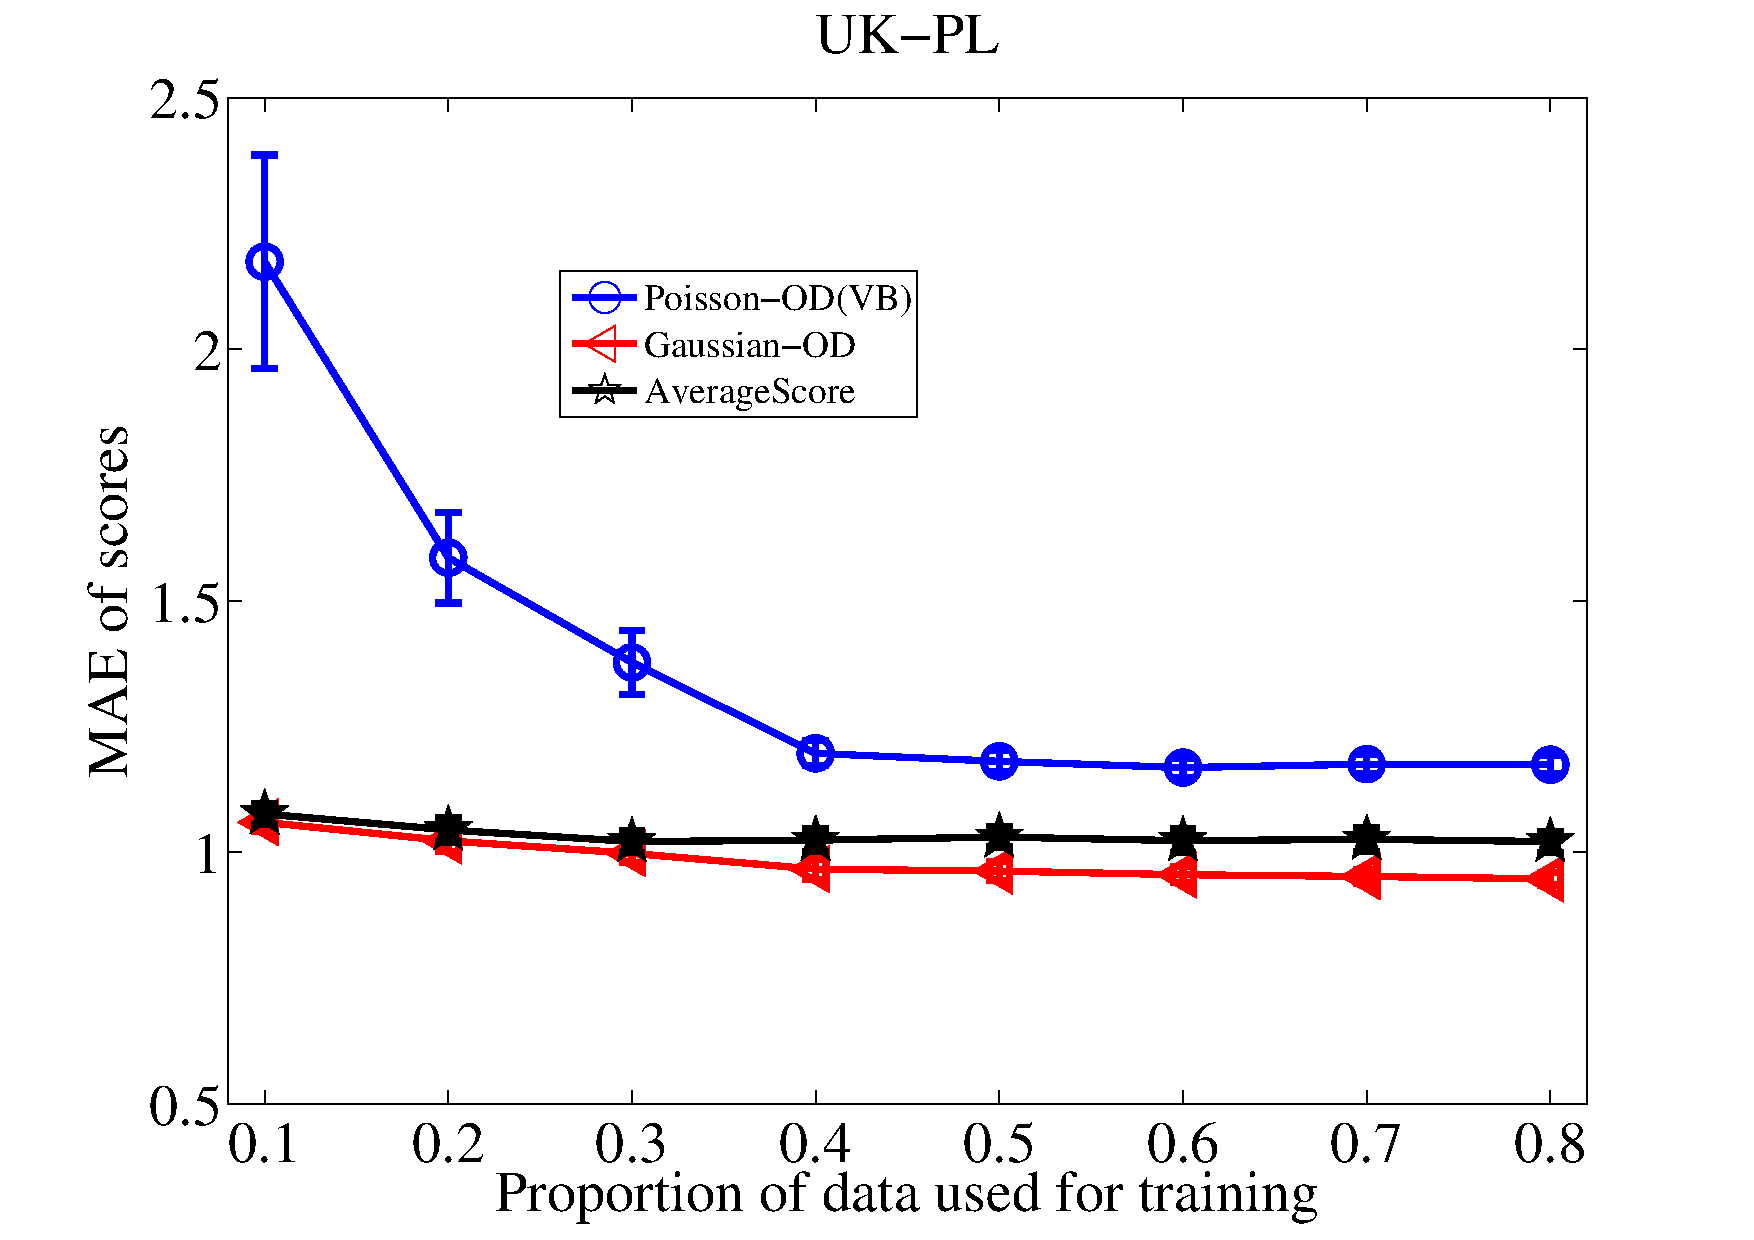
\epsfig{file=ScoreError_UK, angle=0, height=3.6cm}
 }\\
 \subfigure{
    \hspace{-1.2cm}
   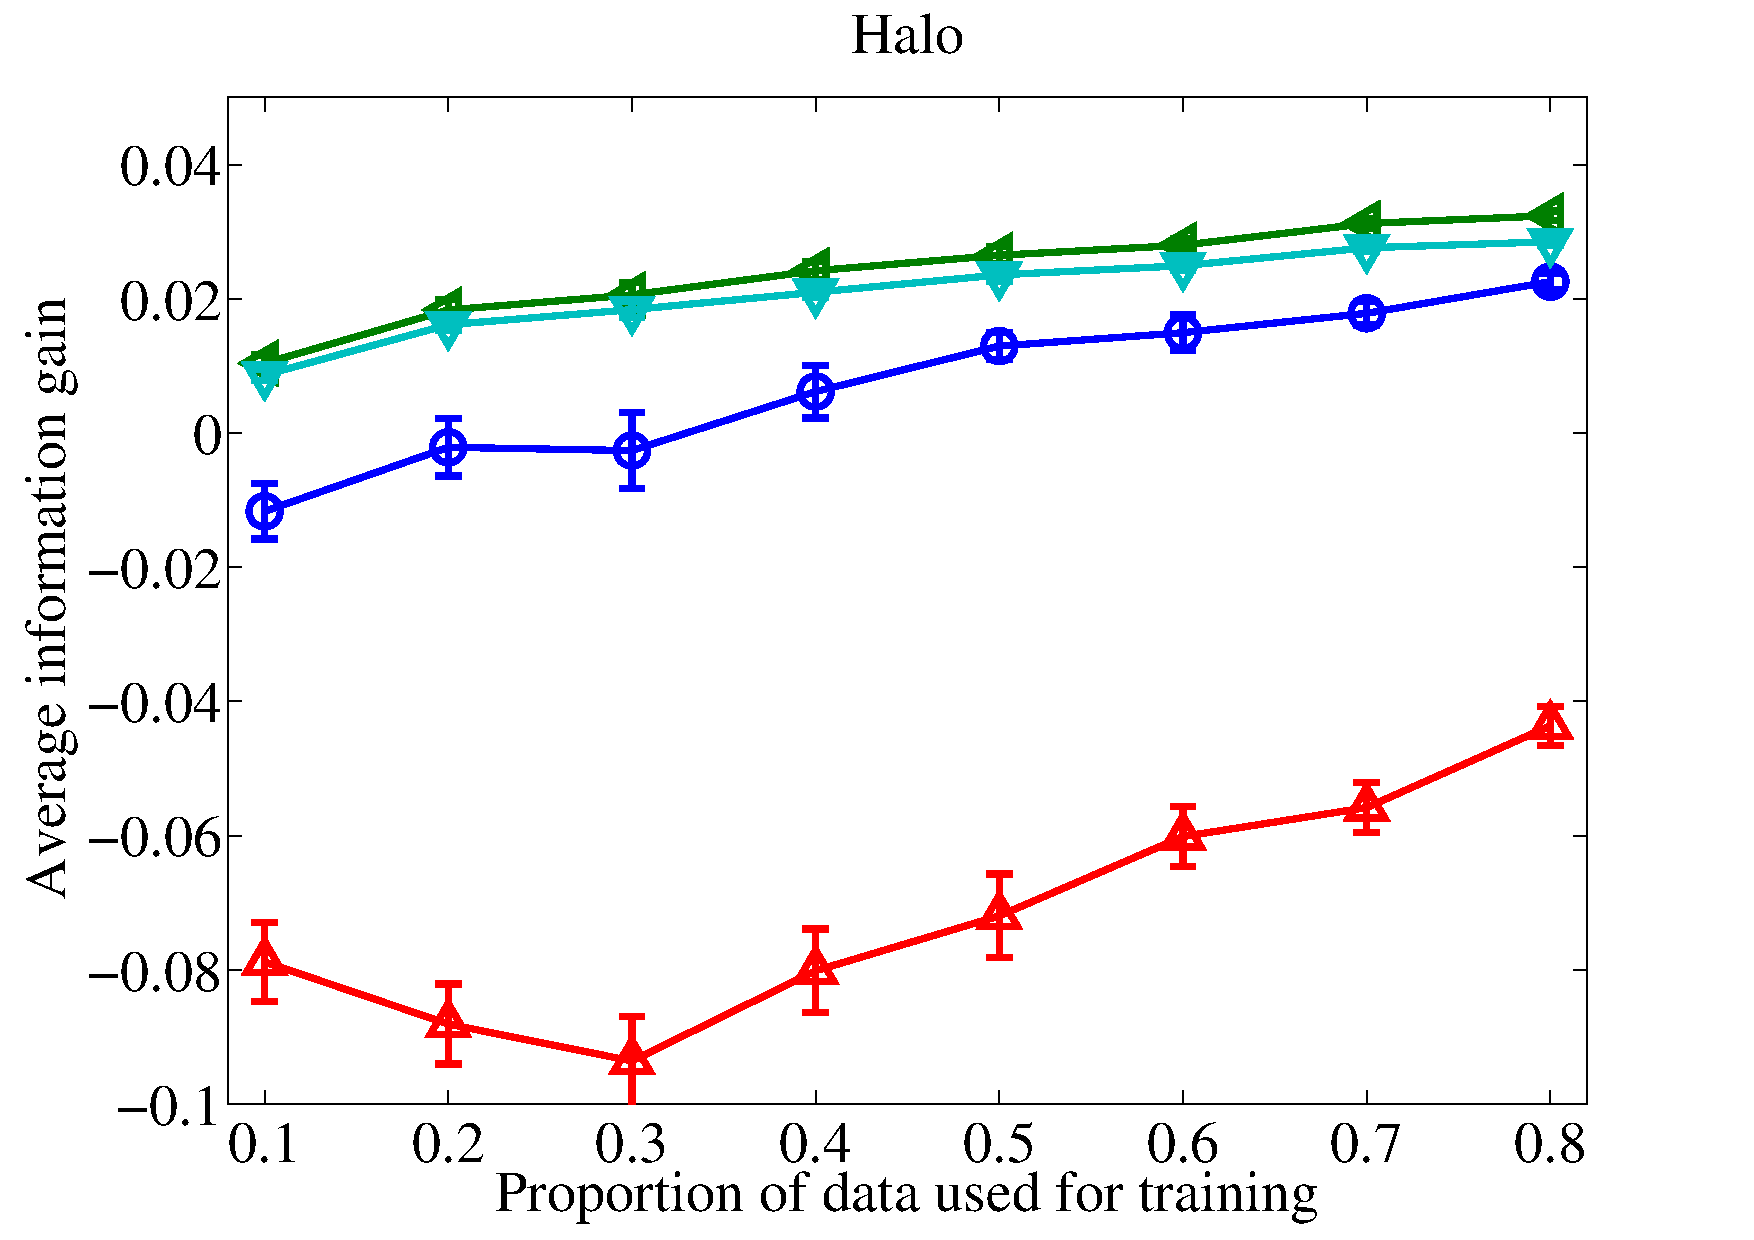
\epsfig{file=InforGain_Halo, angle=0, height=3.6cm}
   \hspace{-0.725cm}
   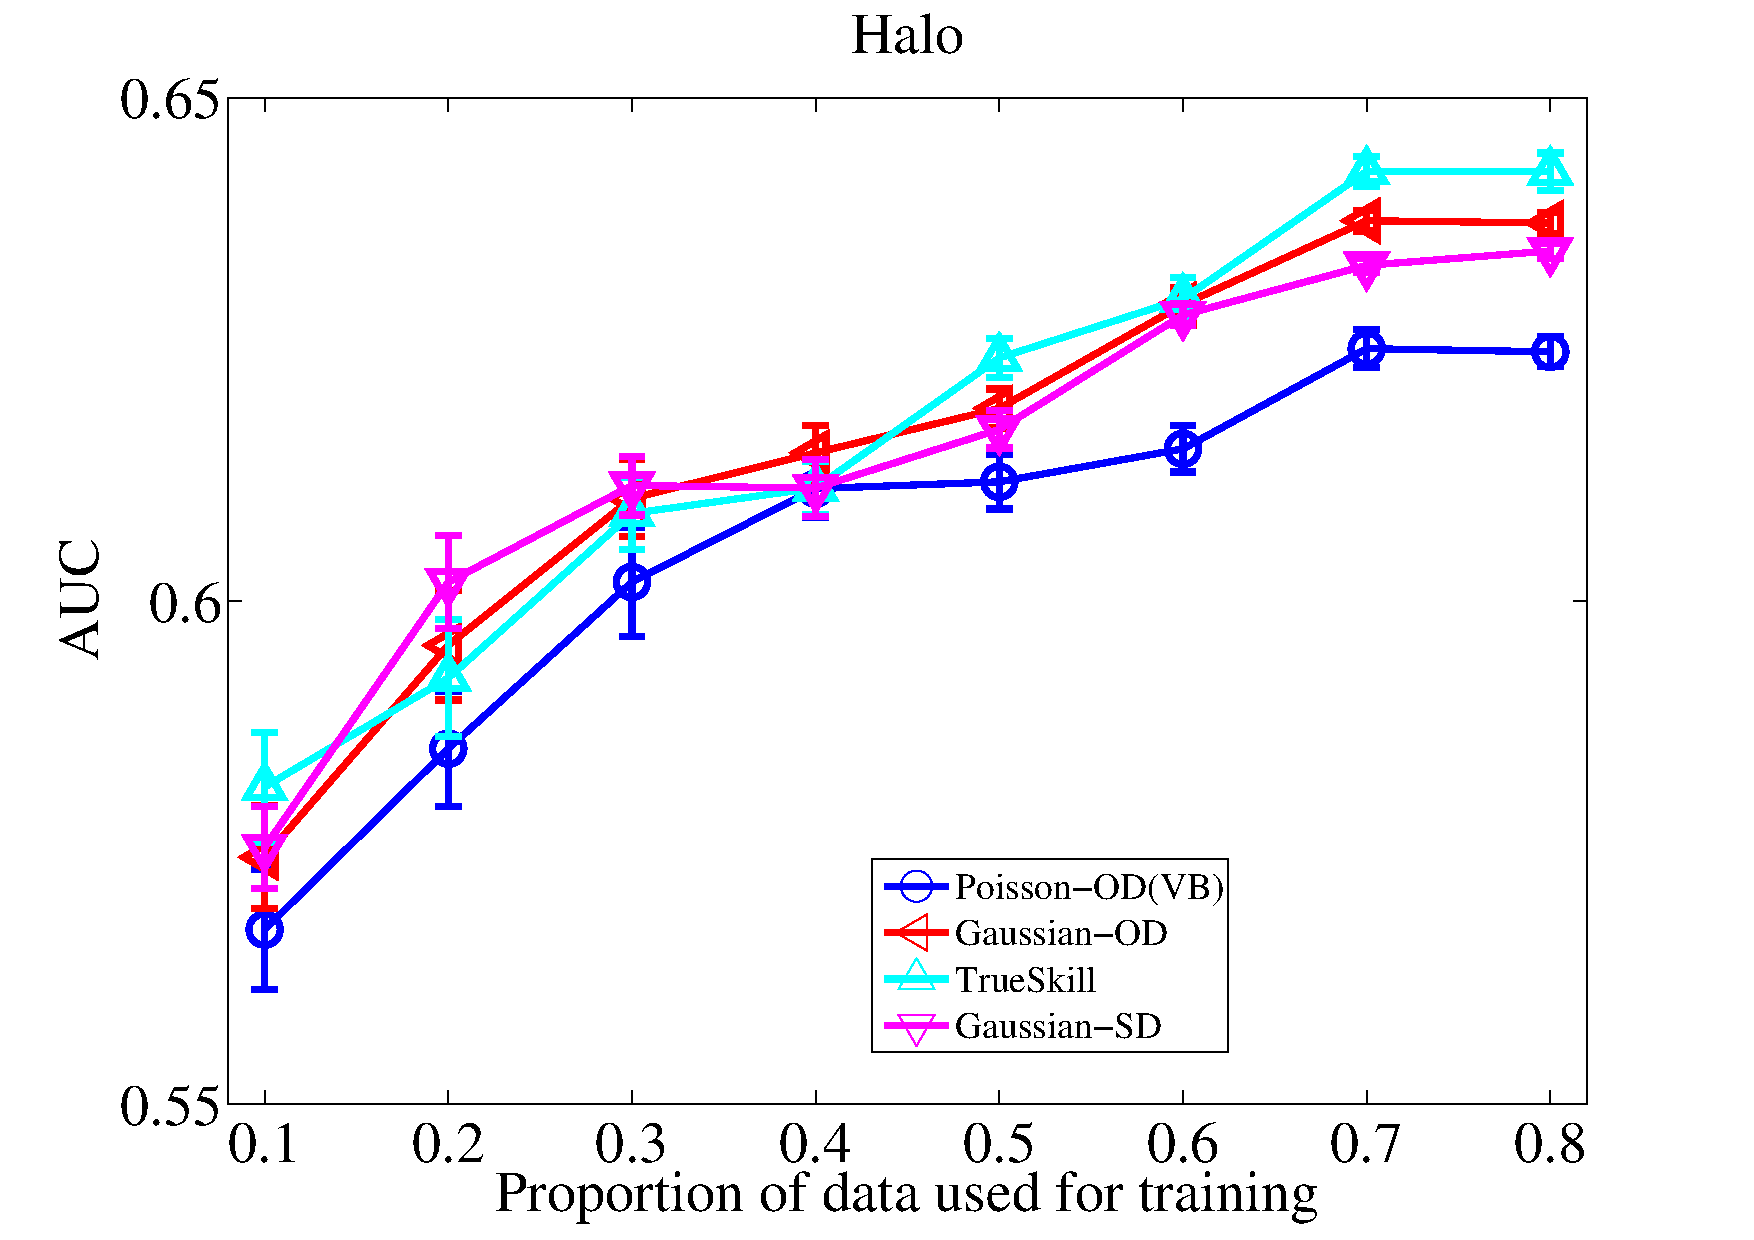
\epsfig{file=WLAccuracy_Halo, angle=0, height=3.6cm}
   \hspace{-0.725cm}
   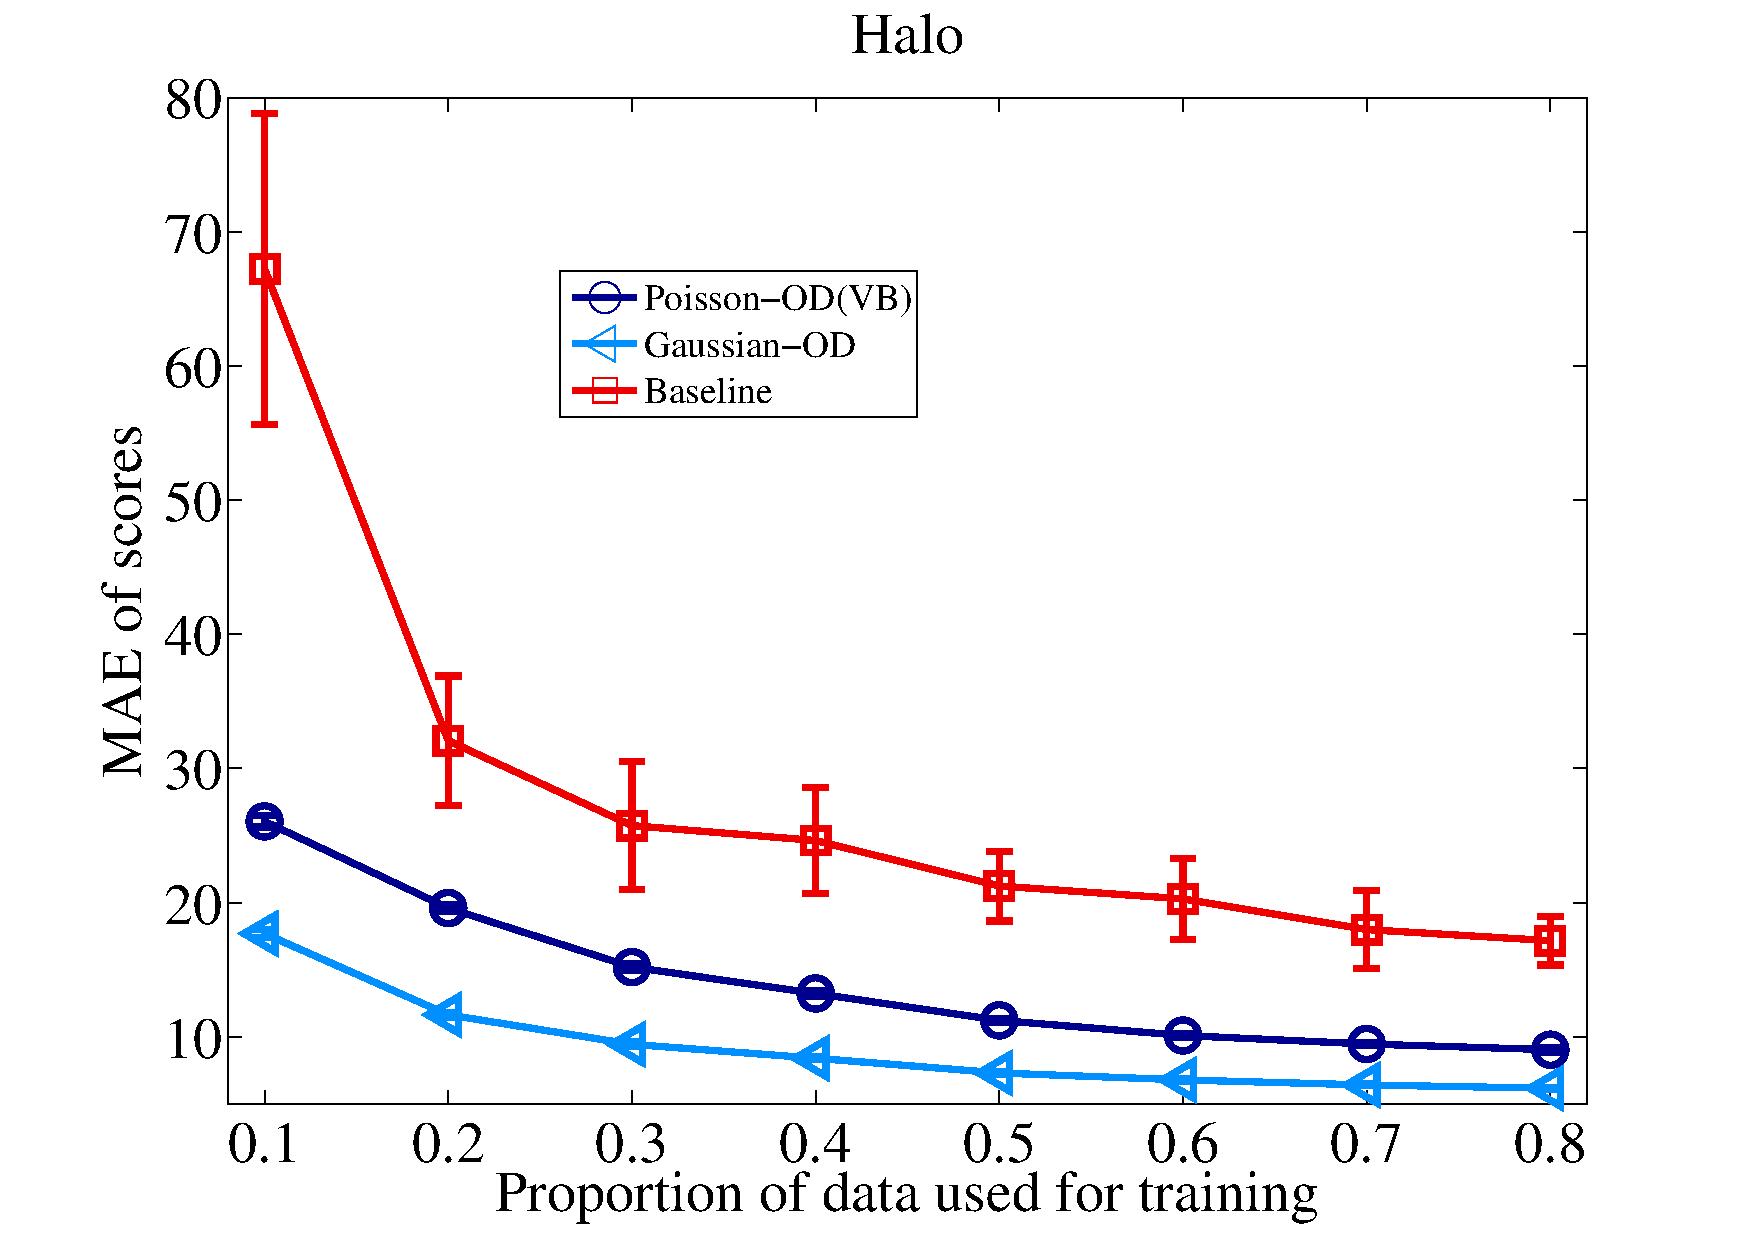
\epsfig{file=ScoreError_Halo, angle=0, height=3.6cm}
 }\\
 \subfigure{
    \hspace{-1.2cm}
   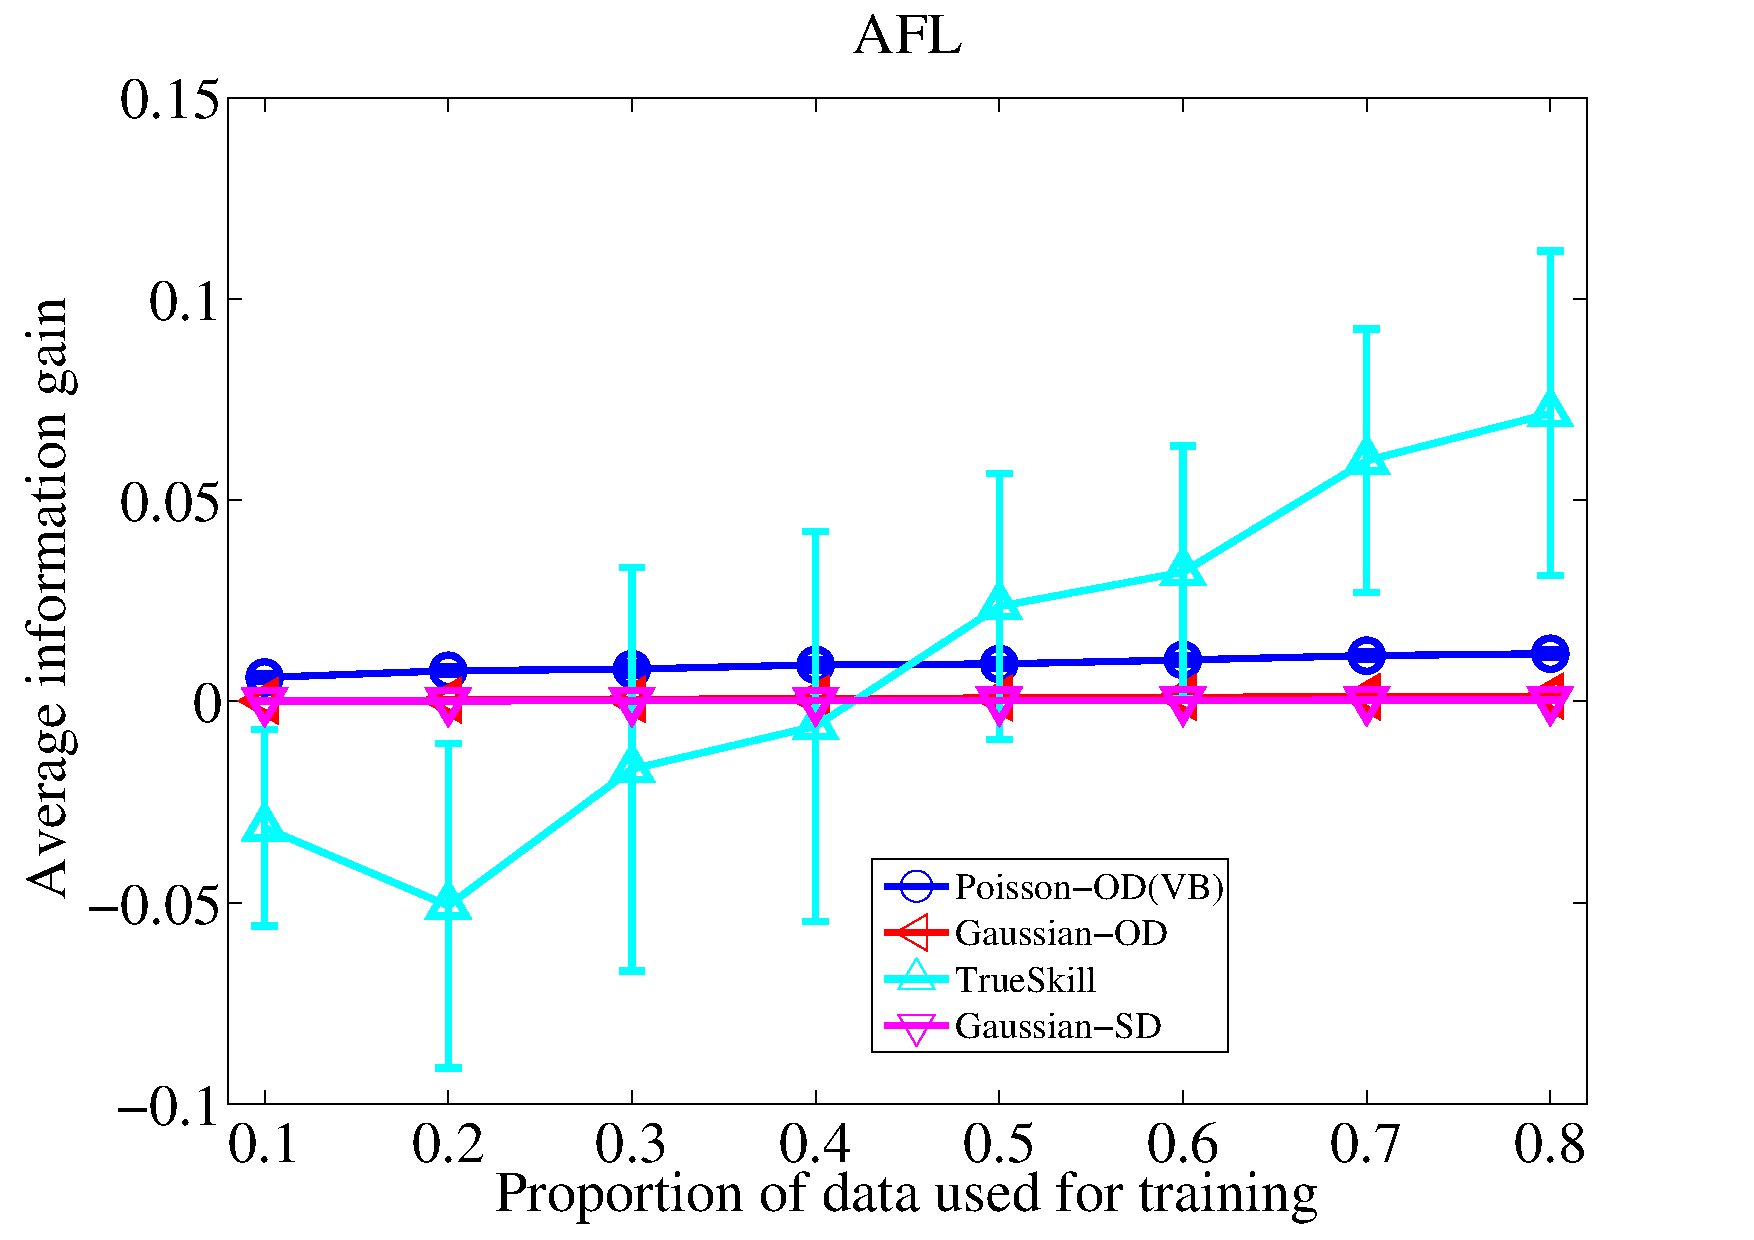
\epsfig{file=InforGain_AFL, angle=0, height=3.6cm}
   \hspace{-0.725cm}
   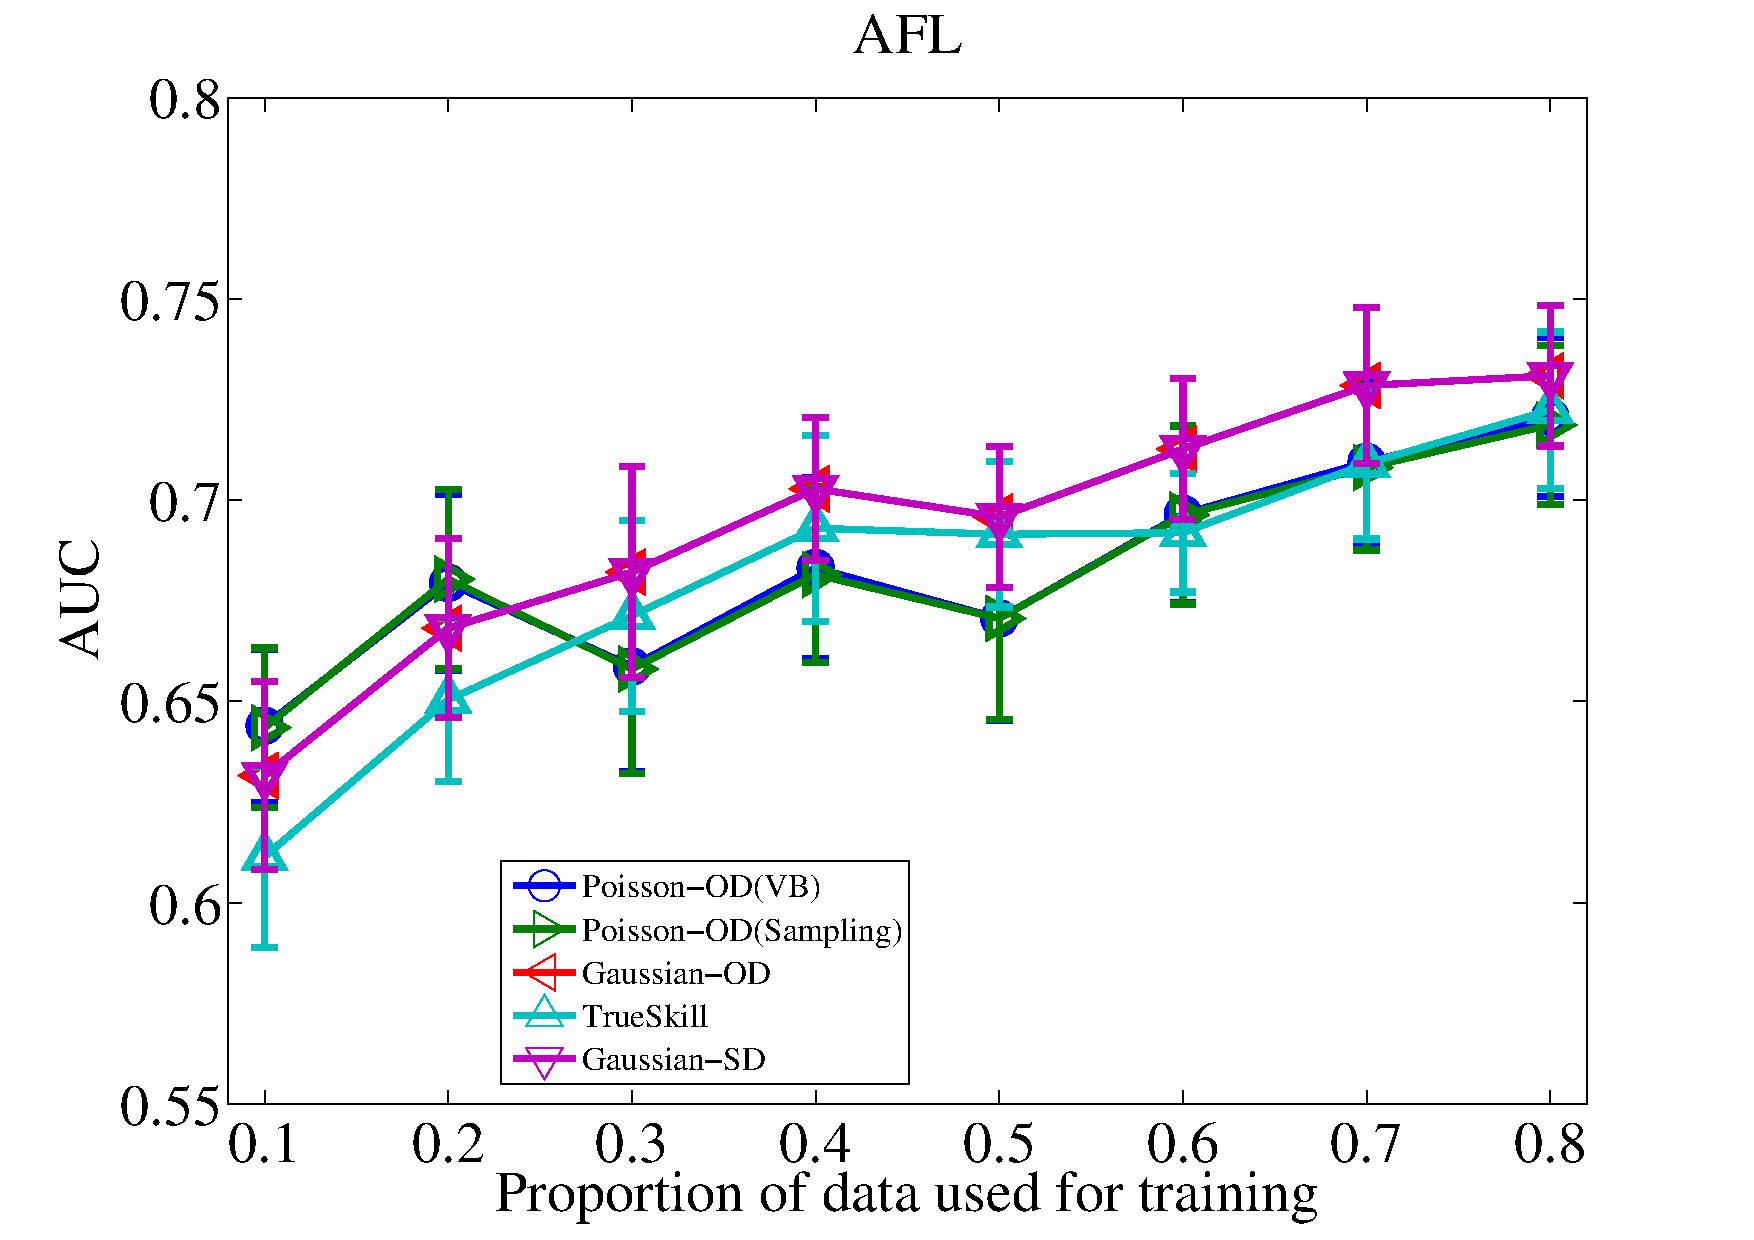
\epsfig{file=WLAccuracy_AFL, angle=0, height=3.6cm}
   \hspace{-0.725cm}
   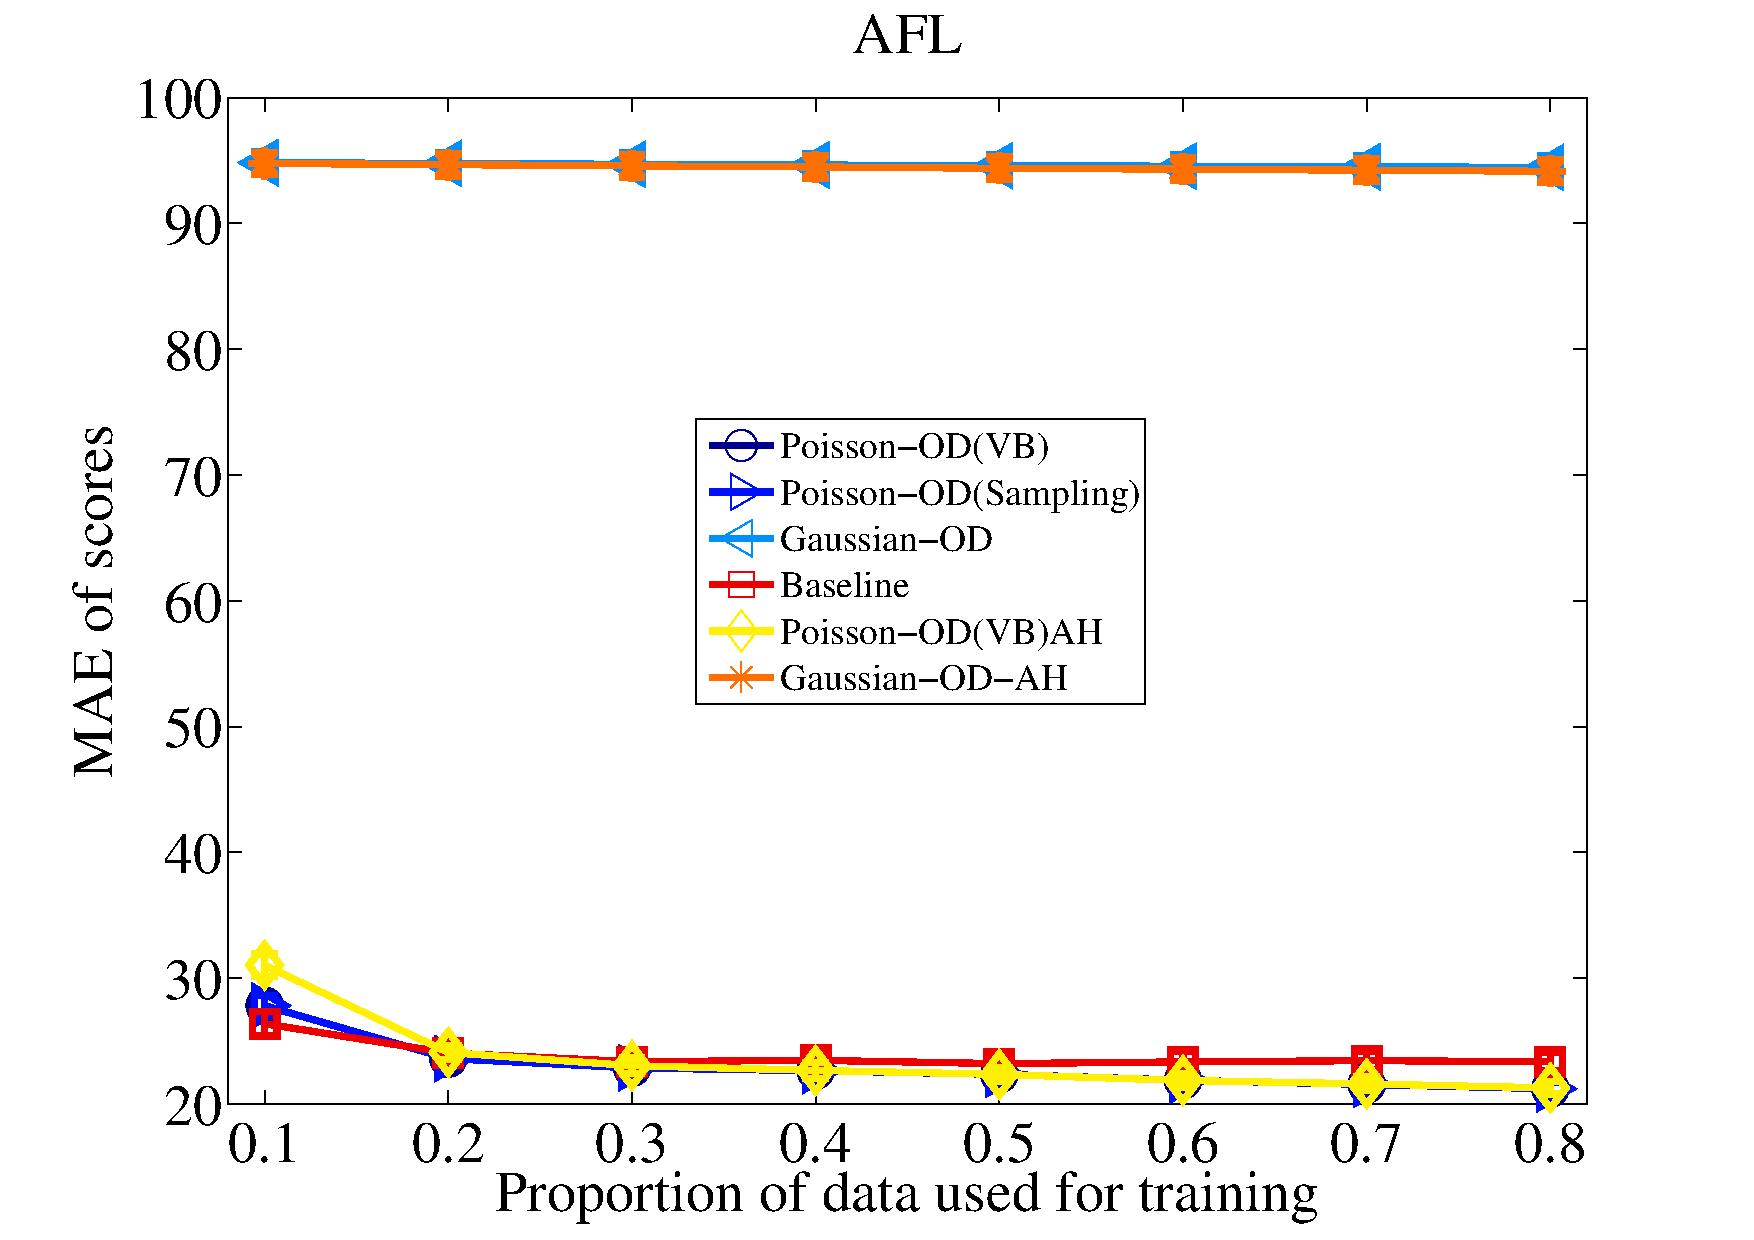
\epsfig{file=ScoreError_AFL, angle=0, height=3.6cm}
 }\\
\vspace{-0.3cm}
\caption{\small Results on the UK-PL, Halo, and AFL datasets evaluated
using information gain (left column), win/loss prediction accuracy in
term of the area of the curve (AUC) (middle column), and score
prediction error (right column).  Error bars indicate
95\% confidence intervals.}
\vspace{-0.3cm}
\label{fig:Results}
\end{figure*}
\end{center}
%%%%%%%%%%%%%%%%%%%%%%%%%%%%%%%%%%%%%%%%%%%%%%%%%%%%%%%%%%%%%%%%%

\subsubsection{Information Gain}
%\paragraph {Information Gain}

%Poisson-OD does not appear to provide accurate probability
%estimates in general -- we conjecture this could be due to biases
%introduced in the variational approximation scheme.
For relatively small amounts of training data (10\% -- 30\%), the
Gaussian models (OD and SD) statistically significantly outperform
TrueSkill and Poisson-OD in terms of win/loss probability accuracy.
On all data sets except AFL, the Gaussian models perform comparably to
TrueSkill for larger amounts of training data.  Gaussian-OD
statistically significantly outperforms Gaussian-SD for Halo 2,
indicating that separate offence/defence modeling helps.

%These results indicate that (a) score information can be very
%useful for making predictions when training data is limited;
%(b) separate offence/defence modeling seem to help Poisson-OD and Gaussian-OD
%outperform Gaussian-SD on Halo, and (c)
%the Poisson-OD model seems to predict more extreme probabilities, which
%can hurt it when its predictions are wrong.

\subsubsection{Win/no-Win Prediction Accuracy }
%\paragraph{Win/Loss Prediction Accuracy}

In terms of win/no-win prediction accuracy,
%Poisson-OD again does not
%generally perform as well as the other models -- we again conjecture
%this may be due to biases introduced in the variational approximation
%scheme.
the Gaussian-OD model generally
provides the best average AUC, followed by Gaussian-SD, then
TrueSkill (with the exception of cases for Halo 2 with more than 40\%
training data where TrueSkill performs best), then Poisson-oD.
Again, we see that
the separate offence/defence skill modeling of Gaussian-OD gives
it a performance edge over the combined skill model of Gaussian-SD.


%We check the statistics of the match outcomes
%(Table~\ref{table:datasetStatistics}),
%and observe that the average
%scores for the UK-PL, Halo, and AFL datasets are 1.3, 42.7, and 95.4,
%respectively.  From this, we might infer the Poisson-OD model predicts better
%when the average scores for a dataset are relatively larger numbers;
%here it seems the exponential term used in the Poisson model can help
%amplify small performance differences to explain high scores, leading
%to more stable skill modeling in high-scoring games.

\subsubsection{Score Prediction Errors}
%\paragraph{Score Prediction Errors}

%For the Gaussian-SD model, we note that the average relative score
%difference error is close 1 indicating the predicted difference is
%probably close to 0 with it being on the correct side of 0 as more
%training data is used.
%The Gaussian-OD model predicts more accurate scores on the UK-PL and
%Halo datasets, and Poisson-OD is more accurate for the AFL dataset.
%This can be explained by a simple skill analysis --- the learned
%skills on the UK-PL dataset tend to show a larger variance (for all
%models), whereas the learned skills on the AFL dataset show little
%variance (for all models except Gaussian-SD).  To confirm our
%previous hypothesis, the use of an exponentiated scoring rate in the
%Poisson model allows it to amplify small performance differences in
%the learned AFL skills to make more accurate score predictions on AFL
%data.  This amplification appears to hurt the Poisson-OD model on the
%relative low-scoring UK-PL dataset.

As shown in the third column in Figure~\ref{fig:Results}, Gaussian-OD
predicts more accurate scores on the UK-PL and Halo datasets, while
Poisson-OD is more accurate for the AFL dataset. This can be explained
by a simple skill analysis --- the learned skills on the UK-PL dataset
tend to show a larger variance (for all models), whereas the learned
skills on the AFL dataset show little variance (for all models except
Gaussian-SD). Thus, the use of an exponentiated scoring rate in the
Poisson-OD model would seem to amplify these small performance
differences in learned AFL skills to make more accurate score
predictions on AFL data.  This amplification appears to hurt the
Poisson-OD model on the lower-scoring UK-PL and Halo dataset (the mean
score for the AFL data is 95.4 vs 42.7 and 1.3 respectively for the
Halo 2 and UK-PL data).

%For the results on the Halo dataset, it is interesting to note that the Gaussian-OD and
%Poisson-OD models slightly outperform the Gaussian-SD model. This can
%perhaps be explained by the strength of modeling offence/defence
%skills separately. Note that both the Gaussian-OD and Poisson-OD
%models propose to treat offence and defence skills separately,
%contrasted with the Gaussian-SD model that uses a single skill
%variable.

\COMMENT
By referring to the score
statistics in Table~\ref{table:datasetStatistics}, our {\it
hypothesis} is that {\it the Poisson model is appropriate for
predicting scores when the match outcomes are given as relatively
larger numbers, which can be explained by its exponentiated rate that
allows to amplify small skill differences to predict the correct rates
needed for high scoring games}. Likewise the Gaussian model without
the exponentiation performs better for low scoring games.

In order to verify the hypothesis, we show the estimated skills after
training on the AFL and UK-PL dataset in
Figure~\ref{fig:ResultsEstimatedSKills}. On the AFL data set, the
differences across the skills of different teams learnt from the
Poisson model and Gaussian-S are relatively small, which supports the
above hypothesis.

%%%%%%%%%%%%%%%%%%%%%%%%%%%%%%%%%%%%%%%%%%%%%%%%%%%%%%%%%%%%%%%%%
\begin{figure*}[t!]
 \centering
 \vspace{-3cm}
 \subfigure{
   \hspace{-0.5cm}
   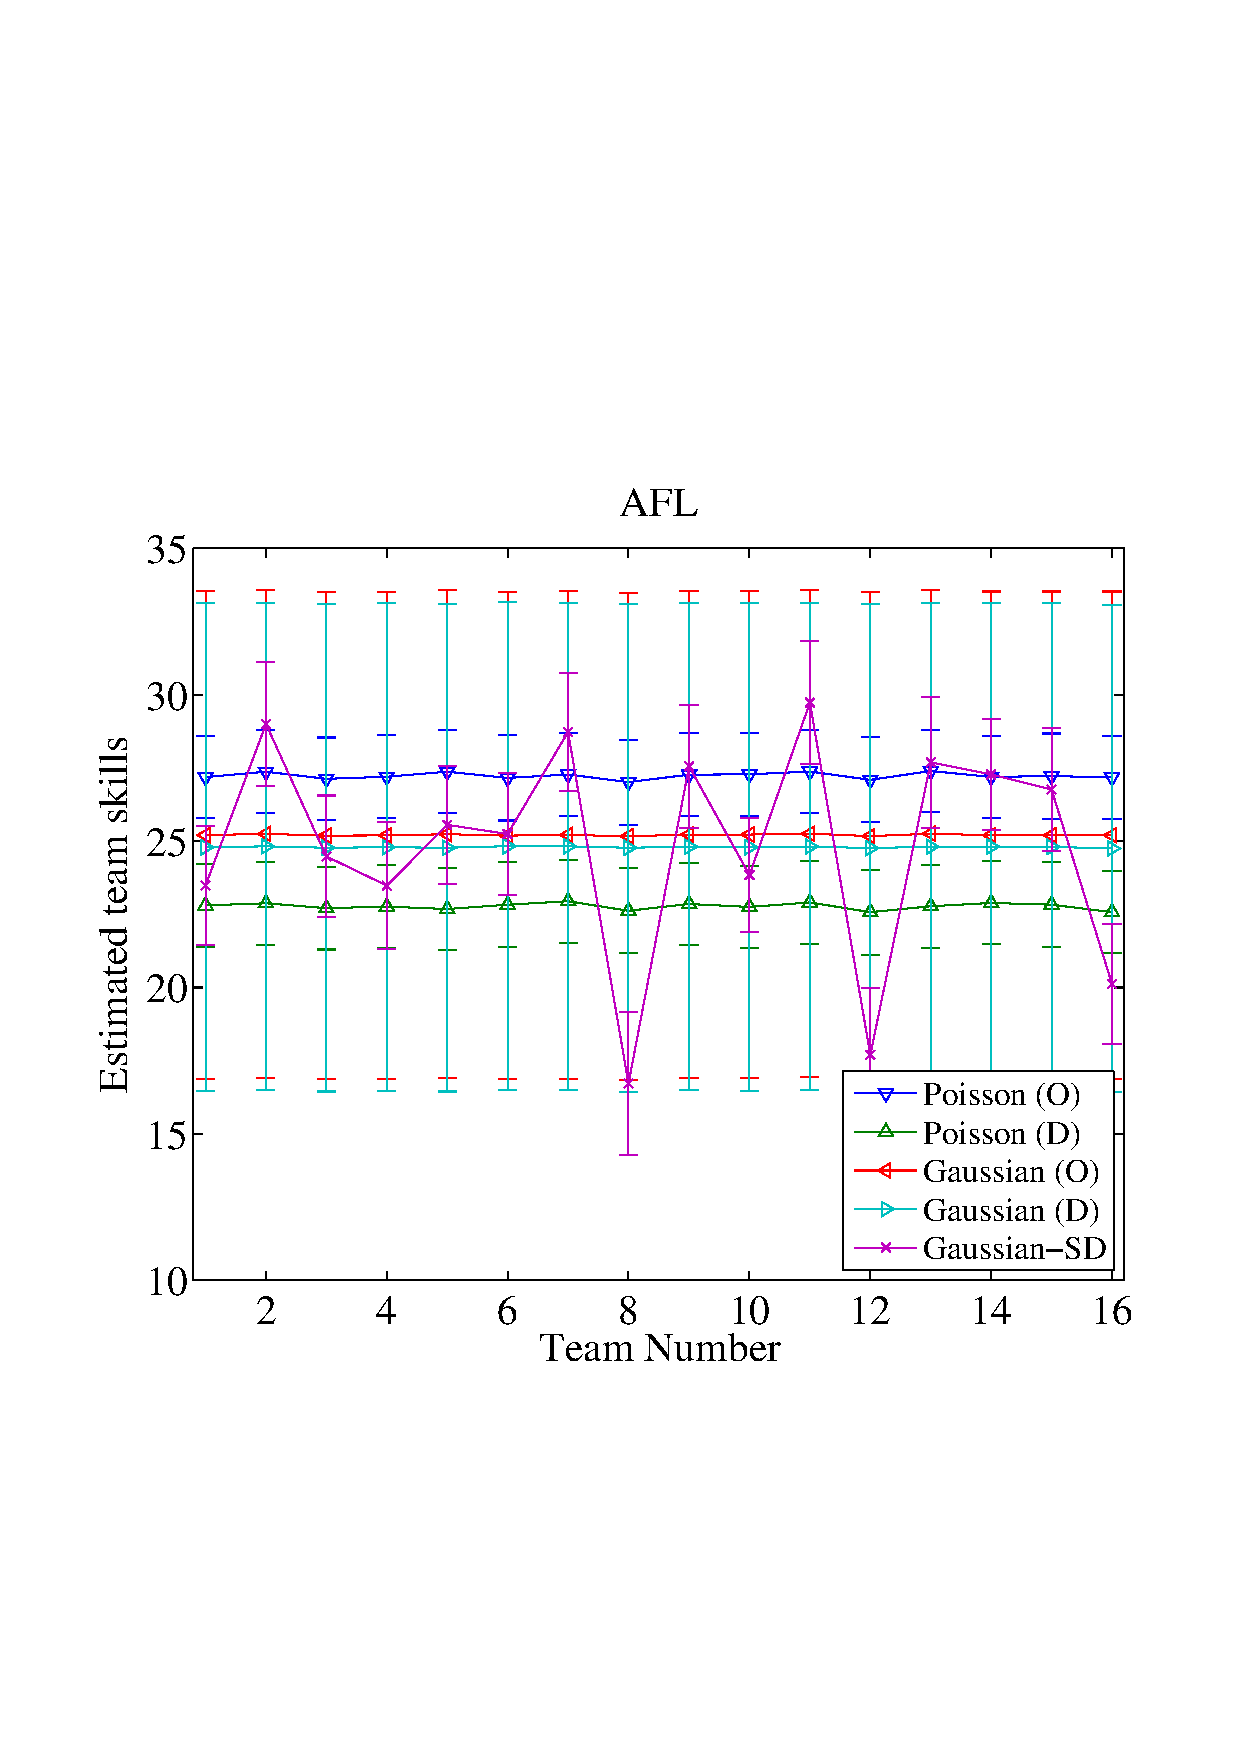
\epsfig{file=skillEstimation_AFL, angle=0, height=13cm}
  \hspace{-1.2cm}
   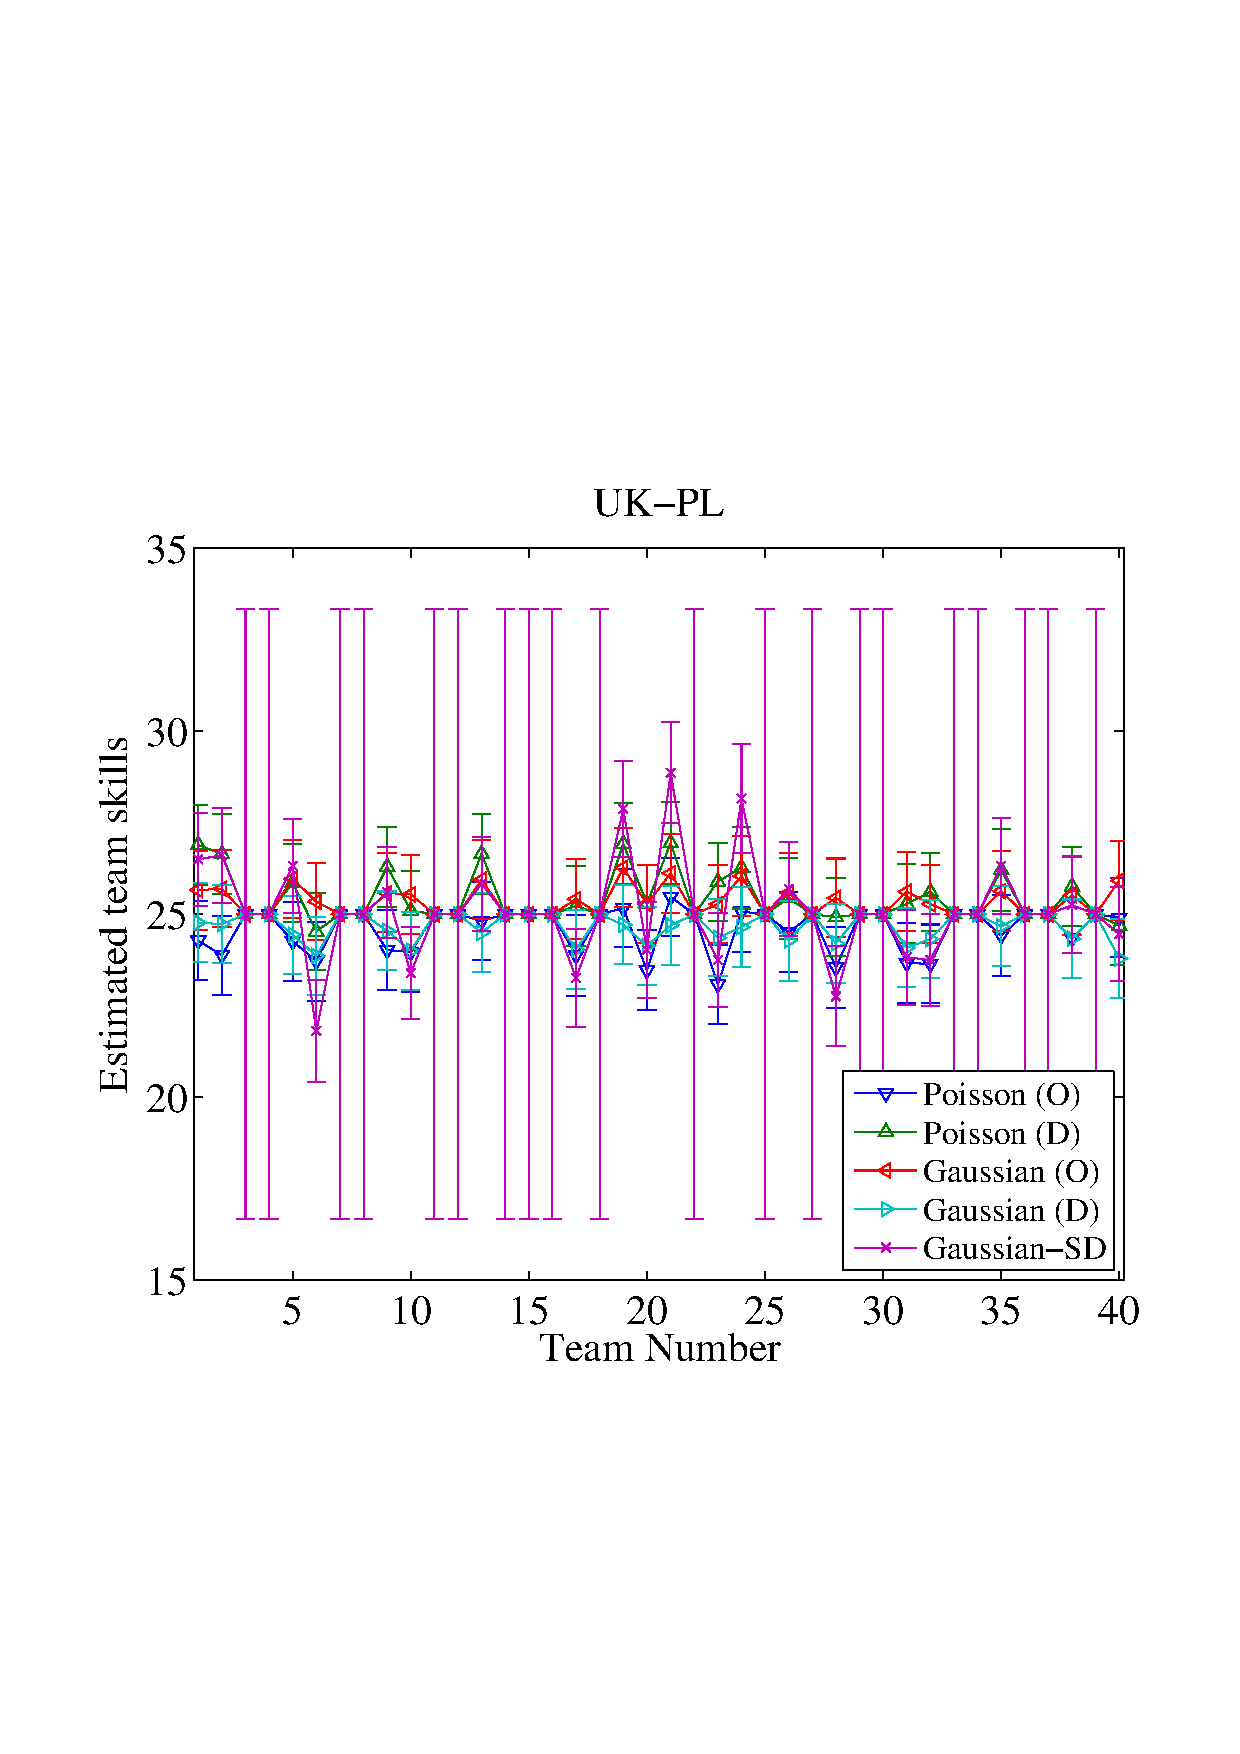
\epsfig{file=skillEstimation_UK, angle=0, height=13cm}
 }\\
 \vspace{-1.5cm}
\caption{Estimated skill levels of teams on the AFL (left) and UK-PL
  data (right) sets. Error bar indicates standard deviation.}
\label{fig:ResultsEstimatedSKills}
\end{figure*}
%%%%%%%%%%%%%%%%%%%%%%%%%%%%%%%%%%%%%%%%%%%%%%%%%%%%%%%%%%%%%%%%%

\ENDCOMMENT


\COMMENT
% JUST THREE NUMBERS, DON'T NEED A TABLE
%%%%%%%%%%%%%%%%%%%%%%%%%%%%%%%%%%%%%%%%%%%%%%%%%%%%%%%%%%%%%%%%%
\begin{table}
\caption{Score statistics for Halo, UK-PL, and AFL}
\begin{center}
\small
\begin{tabular}{|l|c|c|}
  \hline
  % after \\: \hline or \cline{col1-col2} \cline{col3-col4} ...
  Data set          & Mean and Standard Deviation\\
  \hline
  UK-PL             &  1.3023$\pm$1.2237 \\
  Halo 2 Beta     & 42.6929$\pm$3.0440 \\
  AFL                 &95.3784$\pm$27.8993 \\
  \hline
\end{tabular}
\label{table:datasetStatistics}
\end{center}
\end{table}
%%%%%%%%%%%%%%%%%%%%%%%%%%%%%%%%%%%%%%%%%%%%%%%%%%%%%%%%%%%%%%%%%
\ENDCOMMENT


% %TODO
% \begin{itemize}
%   \item Table: {\it testing on the last 10 percent data using models learnt from the first 90 percent data; Five by Three (algorithm by datasets);}
%   \item Performance vs. update \#: {\it testing on the last 10 percent data using models learnt from the first ${0.1, \cdots, 0.9}$ portion of the whole data set, for three data set -- 3 figures.}
%   \item Team rankings vs. o+d ranking (parallel lists in a table): {\it AFL and UK-PL give team ranking after each season. I will only evaluate on the team ranking for the last season. Two tables: one for AFL; the other for UK-PL.}
%   \item Score accuracy: {\it Poisson and Gaussian (S) -- score accuracy; Gaussian (SD) -- score difference accuracy;}
%   \item Bar graph predicted/actual win/lose draw: {\it three datasets, five algorithms, plot W/L/D frequency.}
%   \item Rel Info Gain???
% \end{itemize}

\section{Related Work}

{\bf Skill rating} dates at least as far back as the Elo system
\cite{elo78TheRatingOfChessPlayers}, the idea of which is to model the
probability of the possible game outcome as a function of the two
players' skill levels. Players' skill levels are updated after each
game in a way such that the observed game outcome becomes more likely
and the summation of players' ratings remains unchanged.

The Elo system cannot handle the case when three or more teams
participate in one match, a disadvantage addressed by TrueSkill
\cite{herbrich06569}. %Compared with the Elo system, TrueSkill models each
%player's skill by a Gaussian distribution that simply requires
%maintaining its mean and variance and updates these parameters based on
%WLD match outcomes.
Further extensions of TrueSkill incorporate time-dependent
skill modeling for historical data~\cite{dangauthier07337}.

%TrueSkill assumes that skill update just involves those teams
%participating in a match, i.e., other players' skills are not
%effected. To infer entire time series of skills of players, the
%authors in \cite{dangauthier07337} have extended TrueSkill by
%smoothing through time instead of filtering. Note that both consider
%that players' skills are independent.

In \cite{birlutiu07ExpectationPropagation}, the authors model and learn the
correlation between all players' skills when updating skill beliefs, and
develop a method called ``EP-Correlated", contrasted with the
independent assumption on players' skills
(EP-Independent).  Empirically, EP-Correlated outperforms
EP-Independent on professional tennis match results;
this suggests modeling correlations in extensions of the
score-based learning presented here.

These skill learning methods all share a common feature that they are
restricted to model WLD only and have to discard meaningful
information carried with scores.  While we proposed score-based extensions
of TrueSkill in this work; it remains to incorporate other extensions
motivated by this related work.

{\bf Score modeling} has been studied since the 1950s
\cite{Moroney56FactsFromFigures}
\cite{dixon97ModellingAssociationFootball} \cite{Glickman98JASA}
\cite{Karlis03AnalysisOfSportsData}
\cite{karlis09BayesianModellingFootballOutcomes}; one of the most
popular score models is the Poisson model, first presented in
\cite{Moroney56FactsFromFigures}, and this work continues to the
present~\cite{karlis09BayesianModellingFootballOutcomes}. Other
commonly used score models are based on normal distributions
\cite{Glickman98JASA}. However, it appears that most score-based
models do not distinguish offence and defence skills of each team and
the results here indicate that such separate offence/defence skill
models can perform better than univariate models with limited data.

\section{Conclusion}

We proposed novel score-based, online Bayesian skill learning extensions of
TrueSkill that modeled (1) player's offence and defence skills
separately and (2) how these offence and defence skills
interact to generate scores.  Overall these new models --- and
Gaussian-OD (using a separate offence/defence skill model) in particular ---
show an often improved ability to model winning probability and
win/loss prediction accuracy over TrueSkill, especially when the
amount of training data is limited.  This indicates that there is
indeed useful information in score-based outcomes that is ignored by
TrueSkill and that separate offence/defence skill modeling does help
(c.f. the performance of Gaussian-OD vs. Gaussian-SD).  Furthermore,
these new models allow the prediction of scores (unlike TrueSkill),
with the Poisson-OD model and its variational Bayesian update derived
in Section~\ref{sec:PoissonInference} performing best on the
high-scoring AFL data.  Altogether, these results suggest the
potential advantages of score-based Bayesian skill learning over
state-of-the-art WLD-based skill learning approaches like TrueSkill.

Future research could combine the proposed models with
related work that models home field advantage, time-dependent skills,
multi-team games, and correlated skills to utilise score-based
outcomes.
\subsubsection*{Acknowledgments.} We thank Guillaume Bouchard and Onno Zoeter for interesting discussions, and we also thank the anonymous reviwers for their constructive comments, which help to improve the paper. NICTA is funded by the Australian Government as represented by the Department of Broadband, Communications
and the Digital Economy and the Australian Research Council through the ICT Centre of Excellence program.


\begin{thebibliography}{}
%\small
%\setlength{\itemsep}{.25mm}



\bibitem{Abramowitz74HandbookOfMathematical}
M.~Abramowitz and I.~A. Stegun.
\newblock {\em Handbook of Mathematical Functions, With Formulas, Graphs, and
  Mathematical Tables}.
\newblock Dover Publications, New York, 1974.

\bibitem{birlutiu07ExpectationPropagation}
A.~Birlutiu and T.~Heskes.
\newblock Expectation propagation for rating players in sports competitions.
\newblock In {\em ECML-PKDD}, volume 4702 of {\em LNCS}, pages
  374--381. Springer, 2007.

\bibitem{dangauthier07337}
P.~Dangauthier, R.~Herbrich, T.~Minka, and T.~Graepel.
\newblock Trueskill through time: Revisiting the history of chess.
\newblock In {\em NIPS}, pages 337--344. MIT
  Press, Cambridge, MA, 2008.

\bibitem{elo78TheRatingOfChessPlayers}
A.~E. Elo.
\newblock {\em The rating of chess players: past and present}.
\newblock Arco Publishing, New York, 1978.

\bibitem{herbrich06569}
R.~Herbrich, T.~Minka, and T.~Graepel.
\newblock Trueskill$^{TM}$: A {B}ayesian skill rating system.
\newblock In {\em NIPS}, pages 569--576, 2006.

\bibitem{karlis09BayesianModellingFootballOutcomes}
D.~Karlis and I.~Ntzoufras.
\newblock Bayesian modelling of football outcomes: using the skellam's
  distribution for the goal difference.
\newblock {\em IMA Journal of Management Mathematics}, 20(2):133--145, 2009.

\bibitem{kschischang01498}
F.~R. Kschischang, B.~J. Frey, and H.-A. Loeliger.
\newblock Factor graphs and the sum-product algorithm.
\newblock {\em IEEE Transactions on Information Theory}, 47(2):498--519,
  February 2001.

\bibitem{minka01ExpectationUAI}
T.~Minka.
\newblock Expectation propagation for approximate bayesian inference.
\newblock In {\em UAI}, pages
  362--369. Morgan Kaufmann, 2001.

%\bibitem{thomasMinka2001}
%T.~Minka.
%\newblock {\em A family of algorithms for approximate {B}ayesian inference}.
%\newblock PhD thesis, MIT, 2001.

% \bibitem{thomasMinka2001}
% T.~Minka.
% \newblock {\em A family of algorithms for approximate {B}ayesian inference}.
% \newblock PhD thesis, Department of Electrical Engineering and Computer
%   Science, MIT, January 2001.

\bibitem{Moroney56FactsFromFigures}
M.~J. Moroney.
\newblock {\em Facts from figures}.
\newblock Penguin Press Science, 3rd edition, 1956.

\bibitem{Skellam46TheFrequencyDistribution}
J.~G. Skellam.
\newblock The frequency distribution of the difference between two
{P}oisson variates belonging to different populations.
\newblock {\em Journal of the Royal Statistical Society: Series A}, 109(3):296,
  1946.

\bibitem{Glickman98JASA}
M.~E. Glickman, and H.~S. Stern.
\newblock A state-space model for football league scores.
\newblock {\em Journal of the American Statistical Association}, 93(441):25--35,
  1998.

\bibitem{Beal:EMFixedPoint02}
M.~J. Beal, and Z.~Ghahramani.
\newblock The Variational {B}ayesian {EM} Algorithm for Incomplete Data: with
	Application to Scoring Graphical Model Structures.
\newblock {\em Proceedings of the Seventh Valencia International Meeting}: 453--464,
2002.

\bibitem{karlis09BayesianModellingFootballOutcomes}
D.~Karlis and I.~Ntzoufras,
\newblock Bayesian modelling of football outcomes: using the {S}kellam's distribution
	for the goal difference,
\newblock {\em IMA Journal of Management Mathematics}, 20(2):133--145, 2009.

\bibitem{Karlis03AnalysisOfSportsData}
D.~Karlis and I.~Ntzoufras,
\newblock Analysis of Sports Data by Using Bivariate {P}oisson Models,
\newblock {\em Journal of the Royal Statistical Society: Series D}, 52(3):381-393, 2003.

\bibitem{Moroney56FactsFromFigures}
M.~J. Moroney
\newblock Facts from figures,
\newblock Penguin Press Science, 3rd, 1956.

\bibitem{dixon97ModellingAssociationFootball}
M.~J. Dixon and S.~G. Coles,
\newblock Modelling Association Football Scores and Inefficiencies in the Football Betting Market,
\newblock {\em Journal of the Royal Statistical Society: Series C}, 46(2):265--280, 1997.

%\bibitem{Maragakis08JCP}
%P.~Maragakis and F.~Ritort and C.~Bustamante and M.~Karplus and G.~E.~Crooks
%\newblock Bayesian estimates of free energies from nonequilibrium work data in the presence of instrument noise,
%\newblock {\em Journal of Chemical Physics}, 129(2), 2008.
\end{thebibliography}


%\newpage
%\appendix
%This document is the supplemental material to the ECML-PKDD'12 submission. 
%\section{Exponential Integral}
%\label{app:exponentialIntegral}
%Suppose that $x$ is a random variable with Gaussian distribution, i.e., $p(x):=\mathcal{N}(x; \mu, \sigma^2)$, we present the derivations of the expectation for the $\exp(x)$ w.r.t. $x$ as follows:
%{\small
%\begin{align*}
%    &E_{x\sim p(x)}(\exp(x)) =\int_{x} \frac{\exp(x)}{\sqrt{2\pi \sigma^2}} \exp\left(-\frac{(x-\mu)^2}{2\sigma^2}\right)\mathrm{d}x \\
%    &=\frac{1}{\sqrt{2\pi \sigma^2}} \exp\left(-\frac{\mu^2}{2\sigma^2}\right)\int_{x} \exp\left(-\frac{x^{2}-2x(\mu+\sigma^2)}{2\sigma^2}\right)\mathrm{d}x \\
%    %&=\frac{1}{\sqrt{2\pi \sigma^2}} \exp\left(-\frac{\mu^2}{2\sigma^2}\right) \exp\left(\frac{(\mu+\sigma^2)^2}{2\sigma^2}\right) \int_{x} \exp\left(-\frac{(x-(\mu+\sigma^2))^2}{2\sigma^2}\right)dx\\
%    &=\frac{1}{\sqrt{2\pi \sigma^2}} \exp\left(\mu + \frac{\sigma^2}{2}\right) \int_{x} \exp\left(-\frac{(x-(\mu+\sigma^2))^2}{2\sigma^2}\right)\mathrm{d}x\\
%    &=\frac{1}{\sqrt{2\pi \sigma^2}} \exp\left(\mu + \frac{\sigma^2}{2}\right) \sqrt{2\pi \sigma^2 } \\
%    &=\exp(\mu+\sigma^2/2).
%\end{align*}}
%
%\section{Log Gaussian Integral}
%\label{app:logGaussianIntegral}
%Suppose $x$ is a random variable with Gaussian distribution $p(x): \mathcal{N}\sim(\mu, \sigma^2)$ and $q(x)$ is a Gaussian, $\mathcal{N}\sim(\mu_1, \sigma_1^2)$, let us show how to derive the expectation of $\log q(x)$ w.r.t. $x$ as follows:
%{\small
%\begin{align*}
%    &E_{x\sim p(x)}( \log q(x) ) =E_{x \sim p(x)} \left(\log\left(\frac{1}{\sqrt{2\pi\sigma_1^2}}\exp\left(-\frac{(x-\mu_1)^2}{2\sigma_1^2}\right)\right)\right)\\
%   &= -\frac{1}{2}\log(2\pi\sigma_{1}^2) - \frac{1}{2\sigma_{1}^2}E_{x\sim p(x)}( x-\mu_{1} )^2 \\
%    &= -\frac{1}{2}\log(2\pi\sigma_{1}^2) - \frac{1}{2\sigma_{1}^2}\left(E_{x\sim p(x)}( x^2 )-2\mu_1\mu + \mu_{1}^2 \right) \\
%    &= -\frac{1}{2}\log(2\pi\sigma_{1}^2) - \frac{1}{2\sigma_{1}^2}\left(\sigma^2 + \mu^2-2\mu_1\mu + \mu_{1}^2 \right).
%\end{align*}}
%
%\section{Solution to \eqref{eq:kappa}}
%\label{app:solutionKappa}
%
%First note that \eqref{eq:kappa} is equivalent to
%{\small
%\begin{align*}
%    \frac{1}{2(1+\sigma^2\exp(\kappa))} -\exp(\kappa)& = \frac{\kappa - \mu}{\sigma^2}-s_i,
%\end{align*}
%By setting $z = \exp(\kappa)$ and  $\frac{\kappa - \mu}{\sigma^2}-s_i = A$ , we can convert \eqref{eq:kappa} into a quadratic equation with respect to $z$
%{\small
%\begin{align*}
%    2\sigma^2z^2 + 2(A\sigma^2+1)z+2A-1 = 0,
%\end{align*}}
%with its positive root given by
%{\small
%\begin{align}\label{eq:approximationZQuad4}
%    z & = \frac{-(A\sigma^2+1)+\sqrt{(A\sigma^2-1)^2+2\sigma^2}}{2\sigma^2}.
%\end{align}}
%Note that we choose the positive root because $\exp(\cdot)$ cannot be negative. Given $\frac{\kappa - \mu}{\sigma^2}- s_i = A$ and
%\eqref{eq:approximationZQuad4}, we have
%{\small
%\begin{align}\label{eq:approximationZQuadReplace}
%    z  & =   \frac{\mu + s_i\sigma^2-1-\kappa+\sqrt{(\kappa - \mu - s_i\sigma^2 -1)^2+2\sigma^2}}{2\sigma^2}.
%\end{align}}
%We plug $\exp(\kappa) = z$ into
%\eqref{eq:approximationZQuadReplace}, and get
%{\small
%\begin{align}\label{eq:approximationZQuadAppendix}
%     \kappa  &= \log\left(\frac{\mu + s_i\sigma^2-1-\kappa+\sqrt{(\kappa - \mu - s_i\sigma^2 -1)^2+2\sigma^2}}{2\sigma^2}\right).
%\end{align}}

\end{document}
